\documentclass{article}
\usepackage{fullpage}
\usepackage[utf8]{inputenc}
\usepackage{pict2e}
\usepackage{amsmath}
\usepackage{enumitem}
\usepackage{eurosym}
\usepackage{mathtools}
\usepackage{amssymb, amsfonts, latexsym, cancel}
\setlength{\parskip}{0.3cm}
\usepackage{graphicx}
\usepackage{fontenc}
\usepackage{slashbox}
\usepackage{setspace}
\usepackage{gensymb}
\usepackage{accents}
\usepackage{adjustbox}
\setstretch{1.35}
\usepackage{bold-extra}
\usepackage[document]{ragged2e}
\usepackage{subcaption}
\usepackage{tcolorbox}
\usepackage{xcolor, colortbl}
\usepackage{wrapfig}
\usepackage{empheq}
\usepackage{array}
\usepackage{parskip}
\usepackage{arydshln}
\graphicspath{ {images/} }
\renewcommand*\contentsname{\color{black}Índice} 
\usepackage{array, multirow, multicol}
\definecolor{lightblue}{HTML}{007AFF}
\usepackage{color}
\usepackage{etoolbox}
\usepackage{listings}
\usepackage{mdframed}
\setlength{\parindent}{0pt}
\usepackage{underscore}
\usepackage{hyperref}
\usepackage{tikz}
\usepackage{tikz-cd}
\usetikzlibrary{shapes, positioning, patterns}
\usepackage{tikz-qtree}
\usepackage{biblatex}
\usepackage{pdfpages}
\usepackage{pgfplots}
\usepackage{pgfkeys}
\addbibresource{biblatex-examples.bib}
\usepackage[a4paper, left=1cm, right=1cm, top=1cm,
bottom=1.5cm]{geometry}
\usepackage{titlesec}
\usepackage{titletoc}
\usepackage{tikz-3dplot}
\usepackage{kbordermatrix}
\usetikzlibrary{decorations.pathreplacing}
\newcommand{\Ej}{\textcolor{lightblue}{\underline{Ejemplo}}}
\setlength{\fboxrule}{1.5pt}

% Configura el formato de las secciones utilizando titlesec
\titleformat{\section}
{\color{red}\normalfont\LARGE\bfseries}
{Tema \thesection:}
{10 pt}
{}

% Ajusta el formato de las entradas de la tabla de contenidos
\addtocontents{toc}{\protect\setcounter{tocdepth}{4}}
\addtocontents{toc}{\color{black}}

\titleformat{\subsection}
{\normalfont\Large\bfseries\color{red}}{\thesubsection)}{1em}{\color{lightblue}}

\titleformat{\subsubsection}
{\normalfont\large\bfseries\color{red}}{\thesubsubsection)}{1em}{\color{lightblue}}

\newcommand{\bboxed}[1]{\fcolorbox{lightblue}{lightblue!10}{$#1$}}
\newcommand{\rboxed}[1]{\fcolorbox{red}{red!10}{$#1$}}

\DeclareMathOperator{\N}{\mathbb{N}}
\DeclareMathOperator{\Z}{\mathbb{Z}}
\DeclareMathOperator{\R}{\mathbb{R}}
\DeclareMathOperator{\Q}{\mathbb{Q}}
\DeclareMathOperator{\K}{\mathbb{K}}
\DeclareMathOperator{\im}{\imath}
\DeclareMathOperator{\jm}{\jmath}
\DeclareMathOperator{\col}{\mathrm{Col}}
\DeclareMathOperator{\fil}{\mathrm{Fil}}
\DeclareMathOperator{\rg}{\mathrm{rg}}
\DeclareMathOperator{\nuc}{\mathrm{nuc}}
\DeclareMathOperator{\dimf}{\mathrm{dimFil}}
\DeclareMathOperator{\dimc}{\mathrm{dimCol}}
\DeclareMathOperator{\dimn}{\mathrm{dimnuc}}
\DeclareMathOperator{\dimr}{\mathrm{dimrg}}
\DeclareMathOperator{\dom}{\mathrm{Dom}}
\DeclareMathOperator{\infi}{\int_{-\infty}^{+\infty}}
\newcommand{\dint}[2]{\int_{#1}^{#2}}

\newcommand{\bu}[1]{\textcolor{lightblue}{\underline{#1}}}
\newcommand{\lb}[1]{\textcolor{lightblue}{#1}}
\newcommand{\db}[1]{\textcolor{blue}{#1}}
\newcommand{\rc}[1]{\textcolor{red}{#1}}
\newcommand{\tr}{^\intercal}

\renewcommand{\CancelColor}{\color{lightblue}}

\newcommand{\dx}{\:\mathrm{d}x}
\newcommand{\dt}{\:\mathrm{d}t}
\newcommand{\dy}{\:\mathrm{d}y}
\newcommand{\dz}{\:\mathrm{d}z}
\newcommand{\dth}{\:\mathrm{d}\theta}
\newcommand{\dr}{\:\mathrm{d}\rho}
\newcommand{\du}{\:\mathrm{d}u}
\newcommand{\dv}{\:\mathrm{d}v}
\newcommand{\tozero}[1]{\cancelto{0}{#1}}
\newcommand{\lbb}[2]{\textcolor{lightblue}{\underbracket[1pt]{\textcolor{black}{#1}}_{#2}}}
\newcommand{\dbb}[2]{\textcolor{blue}{\underbracket[1pt]{\textcolor{black}{#1}}_{#2}}}
\newcommand{\rub}[2]{\textcolor{red}{\underbracket[1pt]{\textcolor{black}{#1}}_{#2}}}

\author{Francisco Javier Mercader Martínez}
\date{}
\title{Cálculo II\\ Tema 4: Teoría de campos}

\begin{document}
\maketitle
\textbf{\Large Capítulo 1: Integración múltiple}

\begin{enumerate}[label=\color{red}\textbf{\arabic*)}, leftmargin=*]
\item \lb{Calcular para $\Omega=[0,1]\times[0,3]$ las integrales}
\begin{enumerate}[label=\color{red}\textbf{\alph*)}]
\item $\db{\iint_{\Omega}xy\:\mathrm{d}x\:\mathrm{d}y}$

$\int_{0}^{3}\int_{0}^{1}xy\:\mathrm{d}x\:\mathrm{d}y=\int_{0}^{3}\left[ \dfrac{x^{2}}{2}y \right]_{x=0}^{x=1}\:\mathrm{d}y=\int_{0}^{3}\dfrac{1}{2}y\:\mathrm{d}y=\left[ \dfrac{1}{4}y^{2} \right]_{y=0}^{y=3}=\dfrac{9}{4}$  

\item $\db{\iint_{\Omega}xe^{ y }\:\mathrm{d}x\:\mathrm{d}y}$

$\int_{0}^{3}\int_{0}^{1}xe^{ y }\:\mathrm{d}x\:\mathrm{d}y=\int_{0}^{3}e^{ y }\int_{0}^{1}x\:\mathrm{d}x\:\mathrm{d}y=\int_{0}^{3}e^{ y }\left[ \dfrac{x^{2}}{2} \right]_{x=0}^{x=1}\:\mathrm{d}y=\int_{0}^{3}\dfrac{e^{ y }}{2}\:\mathrm{d}y=\left[ \dfrac{e^{ y }}{2} \right]_{y=0}^{y=3}=\dfrac{1}{2}(e^{ 3 }-1)$

\item $\db{\iint_{\Omega}y^{2}\sin x\:\mathrm{d}x\:\mathrm{d}y}$

$\int_{0}^{3}\int_{0}^{1}y^{2}\sin x\:\mathrm{d}x\:\mathrm{d}y=\int_{0}^{3}y^{2}\left[ -\cos x \right]_{x=0}^{x=1}\:\mathrm{d}y=\int_{0}^{3}y^{2}(1-\cos(1))\:\mathrm{d}y=\left[ \dfrac{y^{3}}{3} \right]_{y=0}^{y=3}\cdot(1-\cos(1))=9(1-\cos(1))$ 

\end{enumerate}

\item \lb{Calcular las integrales dobles siguientes en los recintos que se indican}
\begin{enumerate}[label=\color{red}\textbf{\alph*)}]
\item $\db{\iint_{\Omega}y\:\mathrm{d}x\:\mathrm{d}y\text{ en }\Omega=\{ (x,y)\in\mathbb{R}^{2}: x^{2}+y^{2}\leq 1 \}}$

$\Omega$ es el disco de radio 1 centrado en el origen.

En coordenadas polares, las variables $x$ y $y$ se expresan como: $$
\begin{cases}
x=r\cos\theta\\
y=r\sin\theta\\
\end{cases}\longrightarrow x^2+y^2=r^2
$$

El elemento de área diferencial $\dx\dy$ se transforma en: $$r\dr\dth.$$Los límites de integración en coordenadas polares son: $$r\in[0,1],\quad\theta\in[0,2\pi].$$

$\int_{0}^{2\pi}\int_{0}^{1}r^2\sin\theta\dr\dth=\int_{0}^{2\pi}\left[\dfrac{r^3}{3}\right]_{r=0}^{r=1}\sin\theta\dth=\int_0^{2\pi}\dfrac{1}{3}\cdot\sin\theta\dth=\dfrac{1}{3}\cdot[-\cos\theta]_{\theta=0}^{\theta=2\pi}=\dfrac{1}{3}\left(-\cos(2\pi)+\cos(0)\right)=\dfrac{1}{3}(-1+1)=0$

\item $\db{\iint_{\Omega}(3y^{3}+x^{2})\:\mathrm{d}x\:\mathrm{d}y\text{ en }\Omega=\{ (x,y)\in\mathbb{R}^{2}: x^{2}+y^{2}\leq 1 \}.}$

$\Omega$ es el disco de radio 1 centrado en el origen.

En coordenadas polares, las variables $x$ y $y$ se expresan como: $$
\begin{cases}
x=r\cos\theta\\
y=r\sin\theta\\
\end{cases}\longrightarrow x^2+y^2=r^2
$$
El elemento de área diferencial $\dx\dy$ se transforma en: $$r\dr\dth.$$Los límites de integración en coordenadas polares son: $$r\in[0,1],\quad\theta\in[0,2\pi].$$

En estas coordenadas, la función $2y^3+x^2$ se convierte en:
$$2y^3+x^2=3(r\sin\theta)^3+(r\cos\theta)^2.$$

$\begin{aligned}\iint_{\Omega}(2y^3+x^2)\:\mathrm{d}x\:\mathrm{d}y&=\int_{0}^{2\pi}\int_{0}^{1}(3(r\sin\theta)^3+(r\cos\theta)^2)\cdot r\:\mathrm{d}r\:\mathrm{d}\theta=\int_{0}^{2\pi} \int_{0}^{1} 3r^{4}\sin ^{3}\theta+r^{3}\cos ^{2}\theta \:\mathrm{d}r\mathrm{d}\theta\\ &=\int_{0}^{2\pi}\left[ \dfrac{3r^{5}}{5} \right]_{r=0}^{r=1}\cdot \sin ^{3}\theta+\left[ \dfrac{r^{4}}{4} \right]_{r=0}^{r=1}\cdot \cos ^{2}\theta\:\mathrm{d}\theta =\int_{0}^{2\pi}\dfrac{3}{5}\sin ^{3}\theta+\dfrac{1}{4}\cos ^{2}\theta \:\mathrm{d}\theta=\lb{(\ast)}\end{aligned}$

Usamos que $\sin ^{3}\theta=\sin\theta(1-\cos ^{2}\theta)$ y la simetría de $\sin \theta$ en $[0,2\pi]$ implica que: $$
\int_{0}^{2\pi}\sin ^{3}\theta=0 
$$
Usamos la identidad $\cos ^{2}\theta=\dfrac{1+\cos(2\theta)}{2}$. Entonces: $$
\int_{0}^{2\pi} \cos ^{2}\theta \:\mathrm{d}\theta=\int_{0}^{2\pi}\dfrac{1}{2}\:\mathrm{d}\theta+\int_{0}^{2\pi} \dfrac{\cos(2\theta)}{2}\:\mathrm{d}\theta=\left[ \dfrac{1}{2}\theta \right]_{\theta=0}^{\theta=2\pi}+\dfrac{1}{2}\cancelto{0}{\int_{0}^{2\pi}\cos(2\theta)\:\mathrm{d}\theta}=\pi  
$$
$\int_{0}^{2\pi}\cos(2\theta)\:\mathrm{d}\theta=0$ porque $\cos(2\theta)$ es impar en $[0,2\pi]$.

$\lb{(\ast)=}\dfrac{3}{5}\cdot 0+\dfrac{1}{4}\cdot \pi=\dfrac{\pi}{4}$

\item $\db{\iint_{\Omega}\sqrt{ xy }\:\mathrm{d}x\:\mathrm{d}y\text{ en }\Omega=\{ (x,y)\in\mathbb{R}^{2}: x^{2}+y^{2}\leq 1\}.}$

$\Omega$ es el disco de radio 1 centrado en el origen.

La función $\sqrt{ xy }$ depende del producto $xy$. Observamos que:
\begin{itemize}[label=\textbullet]
\item Si $x>0$ y $y>0$, $\sqrt{ xy }>0$.
\item Si $x<0$ o $y<0$, el signo del producto puede cambiar.
\item En particular, en las regiones donde $x>0$, $y<0$ (o viceversa), el producto $xy<0$, y $\sqrt{ xy }$ no está definida para valores negativos.
\end{itemize}
Debido a que $\sqrt{ xy }$ no está definida en $\mathbb{R}^{2}$ cuando $xy<0$, esta integral \textbf{no se puede calcular} sobre $\Omega$ como está formulada, porque incluye regiones donde $xy<0$.

\item $\db{\iint_{\Omega}ye^{ x }\:\mathrm{d}x\:\mathrm{d}y\text{ en }\Omega=\{ (x,y)\in\mathbb{R}^{2}:0\leq y\leq 1,\,0<x\leq y^{2} \}.}$

$\int_{0}^{1}\int_{0}^{y^{2}}ye^{ x }\:\mathrm{d}x\:\mathrm{d}y=\int_{0}^{1}y\cdot\left[ e^{ x } \right]_{x=0}^{x=y^{2}}\:\mathrm{d}y=\int_{0}^{1}y\cdot \left( e^{ y^{2} }-1 \right)\:\mathrm{d}y=\int_{0}^{1}ye^{ y^{2} }-y\:\mathrm{d}y=\int_{0}^{1}ye^{ y }\:\mathrm{d}y-\int_{0}^{1}y\:\mathrm{d}y=\dfrac{1}{2}(e-1)-\dfrac{1}{2}=\dfrac{1}{2}(e-2)$

$\int_{0}^{1}ye^{ y^{2} }\:\mathrm{d}y=\left\{ \begin{array}{l}u=y^{2} \\ \:\mathrm{d}u=2y\:\mathrm{d}y\end{array} \right\}=\int_{0}^{1}e^{ u }\dfrac{\:\mathrm{d}u}{2}=\dfrac{1}{2}\int_{0}^{1}e^{ u }\:\mathrm{d}u=\dfrac{1}{2}\left[ e^{ u } \right]_{u=0}^{u=1}=\dfrac{1}{2}(e-1)$ 

$\int_{0}^{1}y\:\mathrm{d}y=\left[ \dfrac{y^{2}}{2} \right]_{y=0}^{y=1}=\dfrac{1}{2}$

\item $\db{\iint_{\Omega}y+\log x\:\mathrm{d}x\:\mathrm{d}y\text{ en }\Omega=\{ (x,y)\in\mathbb{R}^{2}:0.5\leq x\leq 1,\,x^{2}\leq y\leq x \}.}$

$$\int_{\frac{1}{2}}^{1}\int_{x^{2}}^{x}y+\log x\:\mathrm{d}y\:\mathrm{d}x$$

$\begin{aligned}
\int_{x^{2}}^{x}y+\log x\:\mathrm{d}y&=\int_{x^{2}}^{x}y\:\mathrm{d}y+\int_{x^{2}}^{x}\log x\:\mathrm{d}y=\left[ \dfrac{y^{2}}{2} \right]_{y=x^{2}}^{y=x}+\left[ y\log x \right]_{y=x^{2}}^{y=x}=\left( \dfrac{x^{2}}{2}-\dfrac{(x^{2})^{2}}{2} \right)+\log x(x-x^{2})\\
&=\dfrac{x^{2}(1-x^{2})}{2}+\log x(x-x^{2})
\end{aligned}$

$\int_{\frac{1}{2}}^{1}\dfrac{x^{2}(1-x^{2})}{2}+\log x(x-x^{2})\:\mathrm{d}x=\lbb{\int_{\frac{1}{2}}^{1}\dfrac{x^{2}(1-x^{2})}{2}\:\mathrm{d}x}{I_{1}}+\dbb{\int_{\frac{1}{2}}^{1}\log x(x-x^{2})\:\mathrm{d}x}{I_{2}}$

$\lb{I_{1}}=\int_{\frac{1}{2}}^{1}\dfrac{x^{2}(1-x^{2})}{2}\:\mathrm{d}x=\dfrac{1}{2}\int_{\frac{1}{2}}^{1}x^{2}-x^{4}\:\mathrm{d}x=\dfrac{1}{2}\left[ \dfrac{x^{3}}{3}-\dfrac{x^{5}}{5} \right]_{x=0.5}^{x=1}=\dfrac{1}{2}\cdot \left( \dfrac{47}{480} \right)=\dfrac{47}{960}$

$\db{I_{2}}=\int_{\frac{1}{2}}^{1}\log x(x-x^{2})\:\mathrm{d}x=\int_{\frac{1}{2}}^{1}x\log x-x^{2}\log x\:\mathrm{d}x=\lb{(\ast)}=\left( -\dfrac{1}{8}\log \left( \dfrac{1}{2} \right) -\dfrac{3}{16} \right)-\left( -\dfrac{1}{24}\log \left(\dfrac{1}{2}\right) -\dfrac{7}{72}\right)=-\dfrac{1}{12}\log \left( \dfrac{1}{2} \right)-\dfrac{13}{144}$
$$\lb{(\ast)}\begin{aligned}
\int_{\frac{1}{2}}^{1} x\log x\:\mathrm{d}x&=\left\{ \begin{array}{ll}
u=\log x & \:\mathrm{d}u=\frac{1}{x}\:\mathrm{d}x \\
\:\mathrm{d}v=x\:\mathrm{d}x & v=\frac{x^{2}}{2}
\end{array} \right\}=\left[ \log x\cdot \dfrac{x^{2}}{2} \right]_{x=0.5}^{x=1}-\int_{\frac{1}{2}}^{1} \dfrac{x^{\cancel{2}}}{2}\cdot \dfrac{1}{\cancel{x}}\:\mathrm{d}x=-\dfrac{1}{8}\log \left( \dfrac{1}{2} \right)-\dfrac{1}{2}\int_{\frac{1}{2}}^{1}x\:\mathrm{d}x\\
&=-\dfrac{1}{8}\log \left( \dfrac{1}{2} \right)-\dfrac{1}{2}\left[ \dfrac{x^{2}}{2} \right]_{x=0.5}^{x=1}=-\dfrac{1}{8}\log \left( \dfrac{1}{2} \right)-\dfrac{3}{16} \\
\int_{\frac{1}{2}}^{1} x^{2}\log x\:\mathrm{d}x&=\left\{ \begin{array}{ll}
u=\log x & \:\mathrm{d}u=\frac{1}{x}\:\mathrm{d}x \\
\:\mathrm{d}v=x^{2}\:\mathrm{d}x & v=\frac{x^{3}}{3}
\end{array} \right\}=\left[ \log x\cdot \dfrac{x^{3}}{3} \right]_{x=0.5}^{x=1}-\int_{\frac{1}{2}}^{1} \dfrac{x^{\cancel{3}}}{3}\cdot \dfrac{1}{\cancel{x}}\:\mathrm{d}x=-\dfrac{1}{24}\log \left( \dfrac{1}{2} \right)-\dfrac{1}{3}\int_{\frac{1}{2}}^{1} x^{2}\:\mathrm{d}x\\
&=-\dfrac{1}{24}\log \left( \dfrac{1}{2} \right)-\dfrac{1}{3}\left[ \dfrac{x^{3}}{3} \right]_{x=0.5}^{x=1}=-\dfrac{1}{24}\log \left( \dfrac{1}{2} \right)-\dfrac{7}{72}
\end{aligned}$$

\end{enumerate}

\item \lb{Calcular las integrales dobles siguientes en los recintos que a continuación se dan:}

\begin{enumerate}[label=\color{red}\textbf{\alph*)}]
\item \db{$\iint_{\Omega}(4-y^{2})\:\mathrm{d}x\:\mathrm{d}y$ en el recinto limitado por las ecuaciones $y^{2}=2x$ e $y^{2}=8-2x$.}

Se nos da el recinto limitado por las curvas: \[ y^{2}=2x\quad\text{e}\quad y^{2}=8-2x \]

\includegraphics[width=0.5\textwidth]{"figures/Figure 1"}

Despejamos $x$ en las dos ecuaciones y obtenemos: \[ \begin{array}{l}
y^2=2x\longrightarrow x=\dfrac{y^2}{2}\\
y^2=8-2x\longrightarrow 2x=8-u^2\longrightarrow x=4-\dfrac{y^2}{2}.
\end{array} \]
Por lo tanto, las fronteras de $x$ están dadas por: \[ x_{\mathrm{izq}}(y)=\dfrac{y^{2}}{2},\qquad x_{\mathrm{der}}(y)=4-\dfrac{y^{2}}{2} \]

Para hallar los límites e $y$, igualamos: \[\dfrac{y^2}{2}=4-\dfrac{y^2}{2}\longrightarrow \dfrac{y^2}{2}+\dfrac{y^2}{2}=4\longrightarrow y^2=4\longrightarrow y=\pm2.\]

Por lo tanto, el recinto está comprendido entre $y=-2$ e $y=2$.

Para calcular la integral, dado un valor de $y$ entre $-2$ y $2$, $x$ varía desde $x=\dfrac{y^2}{2}$ hasta $x=4-\dfrac{y^2}{2}$. Por lo tanto: \[\int_{y=-2}^{y=2}\int_{x=\frac{y^2}{2}}^{x=4-\frac{y^2}{2}}(4-y^2)\dx\dy.\]

$\int_{\frac{y^2}{2}}^{4-\frac{y^2}{2}}4-y^2\dx=(4-y^2)\cdot[x]_{x=\frac{y^2}{2}}^{4-\frac{y^2}{2}}=(4-y^2)\cdot\left(4-\dfrac{y^2}{2}-\dfrac{y^2}{2}\right)=(4-y^2)\cdot(4-y^2)=(4-y^2)^2$

Entonces: 

$\int_{-2}^{2}(4-y^2)^2\dy=\int_{-2}^{2}y^4-8y^2+16\dy=\left[\dfrac{y^5}{5}-\dfrac{8y^3}{3}+16y\right]_{y=-2}^{y=2}=\dfrac{512}{15}$

\item \db{$\iint_{\Omega}(x^{4}+y^{2})\:\mathrm{d}x\:\mathrm{d}y$ en el recinto limitado por $y=x^{3}$ e $y=x^{2}$.}

El recinto está limitado por las curvas: 
		\[ y=x ^{3} \quad \text{e}\quad y=x ^{2} .\]  
		
\includegraphics[width=0.5\linewidth]{"figures/Figure 2"}
		
Primero hallamos, los puntos de intersección: 	
		\[x ^{3}=x ^{2} \longrightarrow x ^{3} -x ^{2} =0 \longrightarrow x ^{2} (1-x)=0 \]
Entonces el recinto en el plano $xy$ está entre $ x=0$ y  $ x=1$.

Para $0<x<1$, comprobamos cuál de las dos curvas está arriba. Tomemos un valor intermedio, por ejemplo $x=\dfrac{1}{2}$ : \[
	y=\left( \frac{1}{2} \right) ^2 =\frac{1}{4}, \quad y=\left( \frac{1}{2} \right)^3=\frac{1}{8}
.\] 
Se ve que $x^2$ está por encima de $x^3$ en este rango. Por tanto, el límite superior en $y$ es  $y=x^2$ y el inferior es $y=x^3$.

El recinto $\Omega$ queda definido por: \[
0\le 1,\quad x^3\le y\le x^2
.\] 
Por tanto, la integral es: \[
	\iint_{\Omega}(x^{4}+y^2)\dx \dy=\int_{0}^{1} \int_{x^3}^{x^2} \left( x^{4}+y^2 \right) \dy\dx  
.\] 

$\int_{x^3}^{x^2}(x^4+y^2)\dy=\left[ x^4y+\dfrac{y^3}{3} \right]_{y=x^{3}}^{y=x^2}=\left(x^{4}(x^{2})+\dfrac{(x^{2})^{3}}{3}\right) -\left(x^{4}(x^{3})+\dfrac{(x^{3})^{3}}{3}\right)=x^{6}+\dfrac{x^6}{3}-x^7-\dfrac{x^9}{3}=\dfrac{4x^6}{3}-x^7-\dfrac{x^9}{3}$

$\iint_{\Omega}(x^{4}+y^2)\dx\dy?\int_{0}^{1}\left(\dfrac{4x^6}{3}-x^7-\dfrac{x^9}{3}\right)\dx=\left[\dfrac{4x^7}{21}-\dfrac{x^8}{8}-\dfrac{x^{10}}{30}\right]_{x=0}^{x=1}=\dfrac{4}{21}-\dfrac{1}{8}-\dfrac{1}{30}=\bboxed{\dfrac{9}{280}}$

\item \db{$\iint_{\Omega}(x+y)\:\mathrm{d}x\:\mathrm{d}y$ en el recinto limitado por $y=x^{3}$ e $y=x^{4}$ con $-1\leq x\leq 1$.}

El recinto está limitado por las curvas: \[ y=x^{3}\quad\text{y}\quad y=x^{4}, \]con $x$ en el intervalo $[-1,1]$. Para cada valor de $x$ entre $-1$ y $1$, $y$ varía entre $x^4$ (curva inferior) y $x^3$ (curva superior).

\includegraphics[width=0.5\linewidth]{"figures/Figure 3"}

\[ \begin{aligned}
\iint_{\Omega}(x+y)\dx\dy&=\int_{-1}^{1}\int_{x^{4}}^{x^{3}}(x+y)\dy\dx=\int_{-1}^{1}\left( x^{4}+\dfrac{x^6}{2}-x^5-\dfrac{x^{8}}{2} \right)\:\mathrm{d}x=\left[ \dfrac{x^{5}}{5} + \dfrac{x^{7}}{14}-\dfrac{x^6}{6}-\dfrac{x^{9}}{18}\right]_{x=-1}^{x=1}\\
&=\left( \dfrac{1}{5}-\dfrac{-1}{5} \right)+\left( \dfrac{1}{14}-\dfrac{-1}{14} \right)-\cancelto{0}{\left( \dfrac{1}{6}-\dfrac{1}{6} \right)}-\left( \dfrac{1}{18}-\dfrac{-1}{18} \right)=\dfrac{2}{5}+\dfrac{1}{7}-0-\dfrac{1}{9}=\bboxed{\dfrac{136}{315}}
\end{aligned} \]

$\int_{x^{4}}^{x^{3}}x+y\dy=\left[xy+\dfrac{y^2}{2}\right]_{y=x^4}^{y=x^3}=\left(x(x^{3})+\dfrac{(x^{3})^2}{2}\right)-\left( x(x^{4})+\dfrac{(x^{4})^{2}}{2} \right)=x^{4}+\dfrac{x^6}{2}-x^5-\dfrac{x^{8}}{2}$

\item \db{$\iint_{\Omega}(2xy^{2}-y)\:\mathrm{d}x\:\mathrm{d}y$ en la región limitada por $y=|x|,\,y=-|x|$ y $x \in[-1,1]$.}

El recinto está definido por las curvas \[ y=|x|,\quad y=-|x| \]con $x\in[-1,1]$.

\includegraphics[width=0.5\textwidth]{"figures/Figure 4"}

Dado que el recinto es simétrico respecto al eje $y$, es conveniente dividir la integral en dos partes: para $x\ge0$ (es decir, $y=x$ y $y=-x$) y para $x<0$.

Sin pérdida de generalidad, integramos para $x\ge0$ y luego multiplicamos por 2: \[ \iint_\Omega(2xy^2-y)\dx\dy=2\int_{0}^{1}\int_{-x}^{x}(2xy^2-y)\dy\dx=2\int_{0}^{1}\dfrac{4x^4}{3}\dx=2\cdot\left[\dfrac{4x^5}{15}\right]_{x=0}^{x=1}=\bboxed{\dfrac{8}{15}} \]
$\begin{aligned}
\int_{-x}^{x}(2xy^2-y)\dy&=\left[\dfrac{2xy^3}{3}-\dfrac{y^2}{2}\right]_{y=-x}^{y=x}=\left(\dfrac{2x(x^{3})}{3}-\dfrac{x^{2}}{2}\right)-\left(\dfrac{2x(-x^{3})}{3}-\dfrac{(-x)^2}{2}\right)=\dfrac{2x^4}{3}-\dfrac{x^2}{2}-\left(-\dfrac{2x^4}{3}-\dfrac{x^2}{2}\right)\\
&=\dfrac{2x^4}{3}+\dfrac{2x^4}{3}-\cancel{\dfrac{x^2}{2}}+\cancel{\dfrac{x^2}{2}}=\dfrac{4x^4}{3}
\end{aligned}$
\end{enumerate}

\item \lb{Calcular la superficie de las siguientes regiones:}
\begin{enumerate}[label=\color{red}\textbf{\alph*)}]
\item \db{Círculo de radio $R$.}

El área $A$ de un círculo de radio $R$ está dado por la fórmula. \[ A=\pi R^2. \] Esto se deduce usando la definición de una integral doble en coordenadas polares, pero vamos a explicarlo paso a paso para que quede claro.
\begin{enumerate}[label=\arabic*)]
  \item Definición del círculo

    Un círculo de radio $R$ está definido como el conjunto de puntos en el plano que cumple \[
    x^2+y^2\le \R^2
    .\] Esto significa que estamos trabajando en el interior del círculo.

  \item Integral doble para calcular el área

    El área del círculo es \[
    A=\iint_{\text{círculo}}1\dx\dy
    .\] 
Aquí el integrando es 1 porque queremos calcular simplemente la cantidad de espacio (superficie del círculo). 

\item Cambiamos a coordenadas polares:

  Las coordenadas polares son ideales para trabajar con círculos porque se basan en el radio $r$ y el ángulo  $\theta$. Las conversiones son:  \[
  x=r\cos\theta, \quad y=r\sin \theta, \quad \dx\dy=r \dr \dth
.\]
En coordenadas polares:
\begin{itemize}[label=\textbullet]
  \item $r$ varía de  $0$ a  $R$ (desde el centro hasta el borde del círculo).
  \item  $\theta$ varía de  $0$ a  $2\pi$ (un giro completo alrededor del círculo).
\end{itemize}
Por lo tanto, el área se convierte en: \[
A=\int_{0}^{2\pi}\int_{0}^{R}1\cdot r \dr \dth      
.\] 
\item Resolver la integral

  Primero integramos respecto a $r$:  \[
  \int_{0}^{R}r \dr=\left[ \dfrac{r^2}{2} \right]_{0}^{R}=\dfrac{R^2}{2}   
  \] 
  Luego respecto a $\theta$:
   \[
     \int_{0}^{2\pi}\dfrac{R^2}{2}\dth=\dfrac{R^2}{2}\int_{0}^{2\pi} 1\dth=\dfrac{R^2}{2}\cdot [\theta ]_{0}^{2\pi}=\dfrac{R^2}{\cancel{2}}\cdot \cancel{2}\pi = \bboxed{\pi R^2}  
  .\]
\end{enumerate} 

\item \db{Elipse de semiejes $a,b$.}

  Para calcular la superficie de una elipse con semiejes $a$ y  $b$, usamos la fórmula clásica que viene de la geometría:  \[
  \text{Área de la elipse }=\pi ab
  .\] 
  \begin{enumerate}[label=\arabic*)]
    \item Definición de la elipse
      La ecuación de la elipse en el plano es: \[
      \dfrac{x^2}{a^2}+\dfrac{y^2}{b^2}=1,
      \] donde:
      \begin{itemize}[label=\textbullet]
        \item $a$ es la longitud del semieje mayor (horizontal si  $a>b$).
        \item $b$ es la longitud del semieje menor (vertical si  $a>b$).
      \end{itemize}
      La elipse es simétrica respecto a ambos ejes, por lo que podemos trabajar con un solo cuadrante y luego multiplicar por 4 para encontrar el área total.

    \item Área usando una integral doble:

      El área de la región se calcula como una integral doble en el recinto delimitado por la ecuación de la elipse. La fórmula general para el área es: \[
      \text{Área}=\iint_{\text{elipse}}1\dx \dy
      .\] 
    \item Cambio a coordenadas polares elípticas:

      Para resolver esta integral, usamos un cambio de coordenadas que "adapta" la forma de la elipse: \[
      x=ar\cos\theta,\quad y=br\sin\theta,
      \]con $r$ en $0$ y $1$, y $\theta$ en $0$ y  $2\pi$. Este cambio de variables transforma la elipse en un círculo unitario en coordenadas $r,\theta$.

      El jacobiano del cambio de variables da un factor $a,b$. Así, la integral se convierte en: \[
        \text{Área}=\int_{0}^{2\pi}\int_{0}^{1}ab\cdot r \dr \dth =ab \int_{0}^{2\pi}\int_{0}^{1} r \dr \dth =ab\cdot \dfrac{1}{\cancel{2}}\cdot \cancel{2}\pi=\bboxed{\pi ab}
      .\] 
    \item Resolviendo la integral:
      \begin{itemize}[label=\textbullet]
        \item Primero integramos respecto a $r$:  \[
        \int_{0}^{1} r \dr =\left[ \dfrac{r^2}{2} \right] _{0}^{1}=\dfrac{1}{2} 
        .\] 
      \item Luego integramos respecto a $\theta$: \[
      \int_{0}^{2\pi}1\dth =2\pi  
      .\] 
      \end{itemize}
  \end{enumerate}
\item \db{La región limitada por las ecuaciones $x^{2}=4y$ y $2y-x-4=0$.}
  \begin{enumerate}[label=\arabic*)]
    \item Identificar las curvas
      \begin{itemize}[label=\textbullet]
        \item $x^2=4y$ es una parábola que se abre hacia arriba.
        \item $2y-x-4=0$ se puede reescribir como  $y=\dfrac{x}{2}+2$, un línea recta.
      \end{itemize}
    \item Encuentro de puntos de intersección.

      Igualamos las dos ecuaciones para encontrar los límites: \[
        \begin{array}{l}
        x^2=4\cdot \left( \dfrac{x}{2}+2 \right) \longrightarrow x^2=2x+8\longrightarrow x^2-2x-8=0\\
        x=\dfrac{2\pm \sqrt{(-2)^2-4\cdot 1\cdot (-8)} }{2\cdot 1}=\dfrac{2\pm\sqrt{36} }{2}=\begin{cases}
          \dfrac{2+6}{2}=4\\
          \dfrac{2-6}{2}=-2
        \end{cases}
        \end{array}
      \] 
    \item Integral para calcular el área.

      La región está entre $x=-2$ y  $x=4$. La curva superior es la línea $y=\dfrac{x}{2}+2$, y la curva inferior es la parábola $y=\dfrac{x^2}{4}$. El área es: \[
        A=\int_{-2}^{4}\left( \dfrac{x}{2} +2-\dfrac{x^2}{4} \right)\dx =\lbb{\int_{-2}^{4} \dfrac{x^2}{2}\dx  }{I_1}+\dbb{\int_{-2}^{4} 2\dx  }{I_2}-\rub{\int_{-2}^{4} \dfrac{x^2}{4}\dx}{I_3}=\lb{(\ast)} = 3+12-6=\bboxed{9}
      \] 

      $\begin{array}{l}
        \lb{I_1}=\int_{-2}^{4}\dfrac{x}{2}\dx =\dfrac{1}{2}\int_{-2}^{4}x\dx=\dfrac{1}{2}\cdot \left[ \dfrac{x^2}{2} \right]_{-2}^{4}=\dfrac{1}{2}\cdot 6=3\\
        \db{I_2}=\int_{-2}^{4}2\dx =2\cdot [x]_{-2}^{4}=12\\
        \rc{I_3}=\int_{-2}^{4}\dfrac{x^2}{4}\dx =\dfrac{1}{4}\int_{-2}^{4}x^2\dx =\dfrac{1}{4}\left[ \dfrac{x^3}{3} \right] _{-2}^{4}=\dfrac{1}{4}\cdot 24=6    
      \end{array}$

  \end{enumerate}
\item \db{La región limitada por las ecuaciones $x+y=5$ y $xy=6$.}

  \begin{enumerate}[label=\arabic*)]
    \item Identificar las curvas:
      \begin{itemize}[label=\textbullet]
        \item $x+y=5$ es una línea recta.
        \item  $xy=6$ es una hipérbola.
      \end{itemize}

    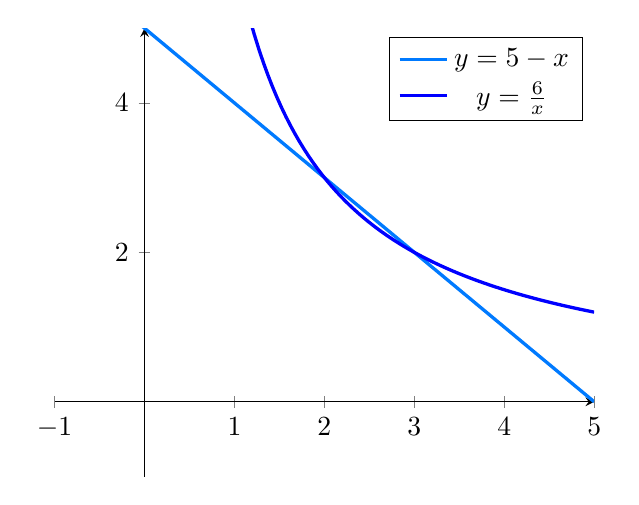
\begin{tikzpicture}
      \begin{axis}[
        xmin= -1, xmax= 5,
        ymin= -1, ymax = 5,
        axis lines = middle,
      ]
        \addplot[domain=-1:5, samples=100, color=lightblue, line width=1.2]{5-x};
        \addlegendentry{$y=5-x$}
        \addplot[domain=0.01:5, samples=100, color=blue, line width=1.2]{6/x};
        \addlegendentry{$y=\tfrac{6}{x}$}
      \end{axis}
    \end{tikzpicture}
  \item Encuentro de puntos de intersección.

    Sustituimos $y=5-x$ en  $xy=6$:  \[
    \begin{array}{l}
      x(5-x)=6\longrightarrow 5x-x^2=6\longrightarrow x^2-5x+6=0\\
      x=\dfrac{5\pm\sqrt{(-5)^2-4\cdot 1\cdot 6}}{2\cdot 1}=\dfrac{5\pm\sqrt{1} }{2}=\begin{cases}
        \dfrac{5+1}{2}=3\\
        \dfrac{5-1}{2}=2
      \end{cases}
    \end{array}
    \] 
  \item Integral para calcular el área.

    La región está entre $x=2$ y  $x=3$. La curva superior es  $y=5-x$, y la curva inferior es  $y=\dfrac{6}{x}$. El área es: \[
    \begin{aligned}
      A=\int_{2}^{3} \left( 5-x-\dfrac{6}{x} \right) \dx& =\left[ 5x-\dfrac{x^2}{2}-6\cdot \ln(x) \right]_{2}^3=5-\dfrac{5}{2}-6\left( \ln(3)-\ln(2) \right)\\
                                                        &= \dfrac{5}{2}-6\left( \ln(3)-\ln(2) \right) =\bboxed{\dfrac{5}{2}-6\ln\left( \dfrac{3}{2} \right) }
    \end{aligned}
    \] 
  \end{enumerate}

\item \db{La región limitada por las ecuaciones $x=y$ y $x=4y-y^{2}$.}
  \begin{enumerate}[label=\arabic*)]
    \item Encontrar los puntos de intersección

      Dadas las ecuaciones: \[
      x=y\quad\text{y}\quad x=4y-y^2
      \] 
      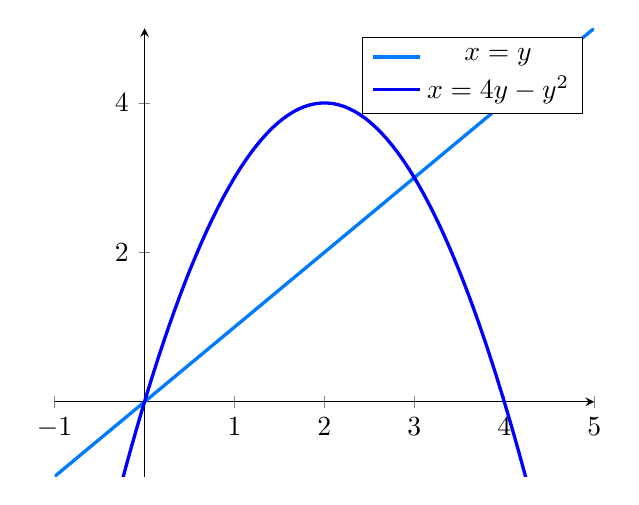
\begin{tikzpicture}
        \begin{axis}[
          xmin= -1, xmax= 5,
          ymin= -1, ymax = 5,
          axis lines = middle,
        ]
          \addplot[domain=-1:5, samples=100, color=lightblue, line width=1.2] {x};
          \addlegendentry{$x=y$};
          \addplot[domain=-1:5, samples=100, color=blue, line width=1.2] {4*x-x^2};
          \addlegendentry{$x=4y-y^2$};
        \end{axis}
      \end{tikzpicture}

      Sustituyendo $x=y$ en  $x=4y-y^2$: \[
      y=4y-y^2\longrightarrow y^2-3y=0\longrightarrow y(y-3)=0 \begin{cases}
        y=0\\
        y=3
      \end{cases}
      \] 
      Para $y=0\to x=0$ y para $y=3\to x=3$. Los puntos de intersección son $(0,0)$ y  $(3,3)$.

    \item Definir la integral

      La curva  $x=y$ se puede escribir como  $x=y$, y la parábola  $x=4y-y^2$ es la superior en el intervalo dado. La región entre $y=0$ y  $y=3$.

      El área es:
       \[
         A=\int_{0}^{3} (4y-y^2-y)\dy =\int_{0}^{3}3y-y^2\dy =\left[\dfrac{3y^2}{2}-\dfrac{y^3}{3} \right] _{0}^3=\dfrac{27}{2}-9=\bboxed{\dfrac{9}{2}}   
      \] 
  \end{enumerate}
\end{enumerate}

\item \lb{Calcular el volumen de los siguientes sólidos:}
\begin{enumerate}[label=\color{red}\textbf{\alph*)}]
\item \db{El limitado por $\dfrac{x}{2}+\dfrac{y}{3}+\dfrac{z}{4}=1$ y los planos de coordenadas.}

  \begin{enumerate}[label=\arabic*)]
    \item Interpretación del problema

      La ecuación $\dfrac{x}{2}+\dfrac{y}{3}+\dfrac{z}{4}=1$ representa un plano en el espacio tridimensional. os planos coordenados $(xy,yz,xz)$ actúan como restricciones, lo que significa que el sólido está contenido en el primer octante.

      Los puntos donde el plano corta los ejes son:
       \begin{itemize}[label=\textbullet]
        \item Eje $x:x=2$ (cuando  $y=0$ y  $z=0$).
        \item Eje  $y:y=3$ (cuando  $x=0$ y  $z=0$).
        \item Eje $z=4$ (cuando  $x=0$ y  $y=0$).
      \end{itemize}
      El sólido es una \textbf{pirámide} con vértice en el origen $(0,0,0)$ y base triangular definida por los puntos  $(2,0,0), (0,3,0)$, y  $(0,0,4)$. 

      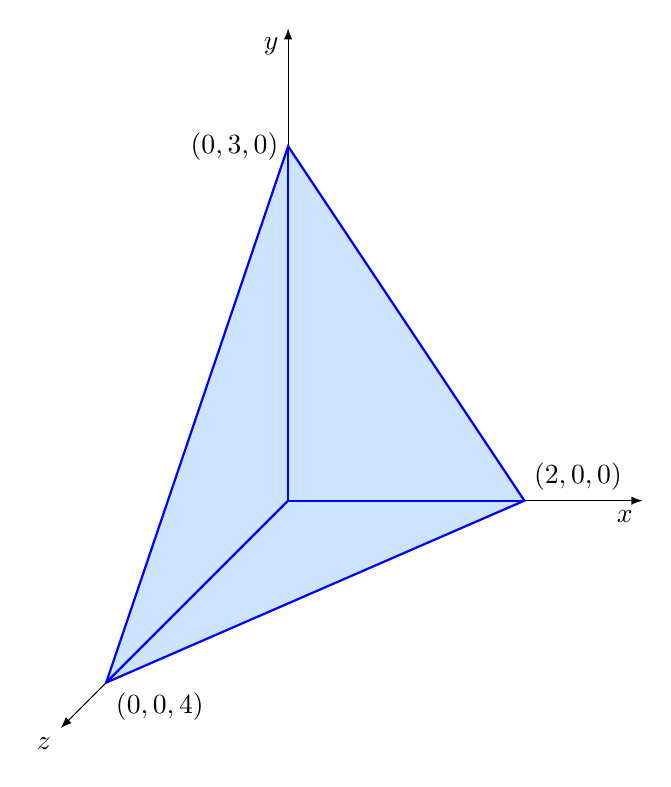
\begin{tikzpicture}[>=latex, scale=1.5]
        \draw[->] (0,0,0) -- (3,0,0) node[anchor=north east] {$x$};
        \draw[->] (0,0,0) -- (0,4,0) node[anchor=north east] {$y$};
        \draw[->] (0,0,0) -- (0,0,5) node[anchor=north east] {$z$};

        \coordinate (O) at (0,0,0);
        \coordinate (A) at (2,0,0);
        \coordinate (B) at (0,3,0);
        \coordinate (C) at (0,0,4);

        \draw[thick, fill=lightblue!20, draw=blue] (A) -- (B) -- (C) -- cycle;

        \draw[thick, blue] (O) -- (A);
        \draw[thick, blue] (O) -- (B);
        \draw[thick, blue] (O) -- (C);
        
        \node[above right] at (A) {$(2,0,0)$};
        \node[left] at (B) {$(0,3,0)$};
        \node[below right] at (C) {$(0,0,4)$};
      \end{tikzpicture}

    \item Fórmula del volumen

      El volumen de una pirámide con base triangular está dado por: \[
        \text{V}=\dfrac{1}{6}\cdot \text{Base}\cdot \text{Altura}.
      \]
      \begin{enumerate}[label=\arabic*)]
        \item \textbf{Base triangular:} La base triangular está en el plano $z=0$, con vértices en  $(2,0), (0,3)$, y  $(0,0)$. El área de un triángulo es:  \[
        \text{Área}=\dfrac{1}{2}\cdot \text{base}\cdot \text{altura}.
        \] 
        Aquí, la base del triángulo es $2$ y la altura es  $3$, así que: \[
        \text{Área}=\dfrac{1}{2}\cdot 2\cdot 3=3.
        \] 
      \item \textbf{Altura de la pirámide:} La altura es la distancia desde el origen al plano en el eje $z$, que es  $4$.
      \item  \textbf{Volumen:} Sustituyendo en la fórmula: \[
          V=\dfrac{1}{6}\cdot 3\cdot 4=\bboxed{2}.
      \]
      \end{enumerate}
  \end{enumerate}
\item \db{El tronco limitado superiormente por $z=2x+3y$ e inferiormente por el cuadrado $[0,1]\times[0,1]$.}

  \begin{enumerate}[label=\arabic*)]
    \item Interpolación del problema

      El sólido está limitado por el plano superior $z=2x+3y$ y por el cuadrado en la base  $x\in [0,1]$ y $y\in [0,1]$. Para calcular el volumen, usamos la integral triple: \[
        V=\int_{0}^{1} \int_{0}^{1} \int_{0}^{2x+3y} 1\dz \dy \dx=\bboxed{\dfrac{5}{2}} .   
      \] 
    \item Resolver la integral

      $\int_{z=0}^{z=2x+3y} 1\dz =\left[ z \right] _{0}^{2x+3y}=2x+3y $ 

      $\int_{y=0}^{y=1}2x+3y\dy =\left[ 2xy+\dfrac{3y^2}{2} \right]_{0}^{1}=2x+\dfrac{3}{2} $ 

      $\int_{x=0}^{x=1}2x+\dfrac{3}{2}\dx =\left[ x^2+\dfrac{3}{2}x \right]_{0}^1=1+\dfrac{3}{2}=\dfrac{5}{2}   $

  \end{enumerate}

\item \db{Esfera de radio $R$.}

  El volumen de una \textbf{esfera de radio $R$} se puede calcular usando la fórmula bien conocida: \[
  V=\dfrac{4}{3}\pi R^3.
  \] 

  Para derivar la fórmula, consideramos que la esfera es un sólido de revolución generado al rotar el semicírculo superior de la ecuación de la esfera $(x^2+y^2=R^2)$ alrededor del eje $x$.
   \begin{enumerate}[label=\arabic*)]
    \item Definir el semicírculo:

      Para $y\ge 0$, la ecuación de la esfera es: \[
      y=\sqrt{R^2-x^2}. 
    \] Este semicírculo tiene límites en $x\in[-R,R]$.

  \item Usar el método de discos para calcular el volumen:

    Al rotar este semicírculo alrededor del eje $x$, el volumen del sólido de revolución se calcula como:  \[
    V=\int_{-R}^{R}\pi y^2\dx .
    \] 
  \item Sustituir $y^2$:

    Como $y^2=R^2-x^2$, la integral se convierte en: \[
    V=\pi \int_{-R}^{R}(R^2-x^2)\dx .  
    \]
  \item Resolver la integral:

    Separando \[
    \int_{-R}^{R}(R^2-x^2)\dx =\int_{-R}^{R}R^2\dx -\int_{-R}^{R} x^2\dx .     
    \] 
    \begin{itemize}[label=\textbullet]
      \item Para el primer término: \[
          \int_{-R}^{R}R^2\dx =R^2 \int_{-R}^{R}1\dx =R^2[x]_{-R}^{R}=R^2(R-(-R))=2R^3.
      \] 
    \item Para el segundo término: \[
    \int_{-R}^{R}x^2\dx =\left[ \dfrac{x^3}{3} \right] _{-R}^{R}=\dfrac{R^3}{3}-\dfrac{-(R^3)}{3}=\dfrac{R^3}{3}-\left( -\dfrac{R^3}{3} \right) =\dfrac{2R^3}{3}.  
    \] 
    \end{itemize}

    Sustituyendo en la integral original: \[
      V=\pi\left( 2R^3-\dfrac{2R^3}{3} \right) =\pi\left( \dfrac{6R^3}{3}-\dfrac{2R^3}{3} \right) =\pi \dfrac{4R^3}{3}\longrightarrow\bboxed{V=\dfrac{4}{3}\pi R^3}
    \] 
  \end{enumerate}
\item \db{Cono de altura $h$ y radio de la base $R$.}

  Para calcular el volumen de un cono de altura $h$ y radio de la base  $R$, usamos la fórmula estándar para que el volumen de un cono, que puede derivarse mediante integración o por la relación con una pirámide.

  El volumen de un cono está dado por: \[
  V=\dfrac{1}{3}\pi R^2h.
  \] Esta fórmula se puede entender como un tercio del volumen de un cilindro con la misma altura y base.

  Imaginemos que el cono está orientado con su vértice en el origen, su eje a lo largo del eje $z$, y su base en  $z=h$. La ecuación de la generatriz del cono es: \[
  r(z)=\dfrac{R}{h}z,
  \] donde $r(z)$ es el radio del círculo en un plano horizontal a una altura  $z$.

  El volumen de un cono puede calcularse integrando los volúmenes de los infinitos discos horizontales:  \[
  V=\int_{0}^{h} \text{área del disco }\dz . 
  \] 
  El área de un disco de una altura $z$ es:  \[
  \text{Área} =\pi r(z)^2=\pi\left( \dfrac{R}{h}z \right) ^2.
  \] 
  Sustituyendo en la integral: \[
  V=\int_{0}^{h} \pi\left( \dfrac{R}{h}z \right) ^2\dz . 
  \] 
  Sacamos constantes fuera de la integral.

 \[
   V=\pi \left( \dfrac{R}{h} \right) ^2 \int_{0}^{h} z^2\dz =\pi\cdot \dfrac{R^2}{h^2}\cdot \left[ \dfrac{z^3}{3} \right] _{0}^{h}=\pi \dfrac{R^2}{\cancel{h^2}}\cdot \dfrac{h^{\cancel{3}}}{3}=\bboxed{\dfrac{1}{3}\pi R^2h} 
 \]  
\item \db{El tronco limitado superiormente por la ecuación $z=2x+1$ e inferiormente por el disco $(x-1)^{2}+y^{2}\leq 1$.}

  El volumen de un sólido se calcula como: \[
 V=\iiint_{\Omega}1\:\mathrm{d}V,
  \] donde la región $\Omega$ es la región tridimensional definida por las restricciones.

  En este caso: 
   \begin{itemize}[label=\textbullet]
    \item El plano superior está dado por $z=2x+1$.
    \item La base del sólido es el disco  $(x-1)^2+y^2\le 1$ en el plano $xy$.
  \end{itemize}
  \begin{enumerate}[label=Paso \arabic*:]
    \item Definir los límites del disco en el plano $xy$

      El disco  $(x-1)^2+y^2\le 1$ tiene centro en $(1,0)$ y radio  $1$. En coordenadas polares:  \[
      x=1+r\cos\theta,\quad y=r\sin\theta,\quad\text{con }0\le r\le 1\text{ y }0\le \theta\le 2\pi.
      \] 
    \item Definir los límites para $z$

      Para un punto en la base, el plano superior tiene la altura:  \[
      z=2x+1.
      \] Por lo tanto: \[
      0\le z\le 2x+1.
      \] 
    \item Calcular el volumen en coordenadas polares

      El volumen se expresa como: \[
      V=\iiint_{\Omega}1\:\mathrm{d}V=\int_{0}^{2\pi} \int_{0}^{1} \int_{0}^{2x+1}1r \dz \dr \dth .    
      \] 
      Aquí, $r$ proviene del cambio a coordenadas polares.

    \item Resolver la integral
      \begin{enumerate}[label=\arabic*)]
        \item Integral respecto a $z$:  \[
            \int_{0}^{2x+1}1\dz =[z]_{0}^{2x+1}=2x+1
        \] 
        Ahora la integral se reduce a: \[
        V=\int_{0}^{2\pi} \int_{0}^{1} (2x+1)r \dr \dth .  
        \] 
      \item Sustituir $x=1+r\cos\theta$:

        En coordenadas polares, $x=1+r\cos\theta$. Sustituyendo: \[
        2x+1=2(1+r\cos\theta)+1=3+2r\cos\theta.
        \] 
        La integral ahora es: \[
        V=\int_{0}^{2\pi}\int_{0}^{1} (3+2r\cos\theta)r \dr \dth = \int_{0}^{2\pi}\int_{0}^{1}(3r+2r^2\cos\theta)\dr \dth .
        \] 
      \item Separar en dos integrales: \[
          V=\int_{0}^{2\pi} \int_{0}^{1} 3r \dr \dth +\int_{0}^{2\pi} \int_{0}^{1} 2r^2\cos\theta\dr \dth = 3\pi + 0 =\bboxed{3\pi}.   
      \] 
    \item Resolver cada integral:
      \begin{itemize}[label=\textbullet]
        \item Para $\int_{0}^{2\pi} \int_{0}^{1}3r \dr \dth$ : \[
        \begin{array}{c}
          \int_{0}^{1} 3r \dr =3\left[ \dfrac{r^2}{2} \right] _{0}^1=\dfrac{3}{2}.\\
          \int_{0}^{2\pi}\dfrac{3}{2}\dth =\dfrac{3}{2}\cdot 2\pi=3\pi.  
        \end{array}
        \] 
      \item Para $\int_{0}^{2\pi} \int_{0}^{1} 2r^2\cos\theta\dr \dth   $ : \[
      \begin{array}{c}
        \int_{0}^{1} 2r^2\dr=2\left[ \dfrac{r^3}{3} \right] _{0}^1=2\cdot \dfrac{1}{3}=\dfrac{2}{3}.\\
        \int_{0}^{2\pi}\dfrac{2}{3}\cos\theta\dth =\dfrac{2}{3}\tozero{\int_{0}^{2\pi}\cos\theta\dth   }=0  
      \end{array}
      \] 
      \end{itemize}
      \end{enumerate}
  \end{enumerate}
\end{enumerate}

\item \lb{Calcular cambiando a coordenadas polares:}

  En coordenadas polares: \[
  x=r\cos\theta,\quad y=r\sin\theta,\quad \dx \dy =r \dr \dth .
  \] 
\begin{enumerate}[label=\color{red}\textbf{\alph*)}]
\item $\db{\int_{-1}^{1}\int_{0}^{\sqrt{ 1-y^{2} }}\sqrt{ x^{2}+y^{2} }\:\mathrm{d}x\:\mathrm{d}y.}$
\begin{enumerate}[label=\arabic*)]
  \item Interpretar la región de integración

    La región está limitada por:
    \begin{itemize}[label=\textbullet]
      \item $y\in [-1,1]$.
      \item $x\in [0,\sqrt{1-y^2}]$
    \end{itemize}
    Esto describe la \textbf{parte superior derecha del círculo de radio 1} centrado en el origen (por $x^2+y^2\le 1$).

    En coordenadas polares: 
    \begin{itemize}[label=\textbullet]
      \item El radio $r$ varía entre  $0$ y  $1$.
      \item El ángulo  $\theta$ varía entre $0$ y  $\dfrac{\pi}{2}$.
    \end{itemize}
  \item Cambiar a coordenadas polares

    \[
      \int_{0}^{\frac{\pi}{2}}\int_{0}^{1} \lbb{\sqrt{r^2\cos^2\theta+r^2\sin^2\theta} }{r}\cdot r \dr \dth =\int_{0}^{\frac{\pi}{2}}r\cdot r \dr \dth =\int_{0}^{\frac{\pi}{2}} r^2\dr \dth .      
    \] 
  \item Resolver la integral

    Primero integramos respecto a $r$:  \[
    \int_{0}^{1} r^2 \dr =\left[ \dfrac{r^3}{3} \right] _{0}^1=\dfrac{1}{3}. 
    \] 
    Luego, integramos respecto a $\theta$:
\[
  \int_{0}^{\frac{\pi}{2}} \dfrac{1}{3} \dth =\dfrac{1}{3}\cdot [\theta]_0^{\frac{\pi}{2}}=\dfrac{1}{3}\cdot \dfrac{\pi}{2}=\bboxed{\dfrac{\pi}{6}}
\] 
\end{enumerate}
\item $\db{\int_{\frac{1}{2}}^{1}\int_{0}^{\sqrt{ 1-x^{2} }}(x^{2}+y^{2})^{\frac{3}{2}}\:\mathrm{d}y\:\mathrm{d}x.}$

  \begin{enumerate}[label=\arabic*)]
    \item Interpretar la región de integración

      La región está limitada por:
      \begin{itemize}[label=\textbullet]
        \item $x \in \left[ \dfrac{1}{2},1 \right] $.
        \item $y\in \left[ 0,\sqrt{1-x^2}  \right] $.
      \end{itemize}
      Esto corresponde a la \textbf{parte superior derecha de un círculo de radio 1}, restringida a $x \in \left[ \dfrac{1}{2},1 \right] $.
      
      En coordenadas polares:
      \begin{itemize}[label=\textbullet]
        \item $r$ varía entre  $\dfrac{1}{2}$ y $1$.
        \item  $\theta$ varía entre $0$ y  $\dfrac{\pi}{2}$.
      \end{itemize}
    \item Cambiar a coordenadas polares

      \[
        \int_{0}^{\frac{\pi}{2} }\int_{\frac{1}{2} }^{1} \lbb{\left(r^2\cos^2\theta+r^2\sin^2\sin\theta \right)^{\frac{3}{2} }}{r^3}    =\int_{0}^{\frac{\pi}{2} }\int_{\frac{1}{2} }^{1}r^3\cdot r\dr \dth =\int_{0}^{\frac{\pi}{2} } \int_{\frac{1}{2} }^{1} r^{4} \dr \dth .
      \] 
    \item Resolver la integral

Primero integramos respecto a $r$:
 \[
\int_{\frac{1}{2} }^{1}r^{4}\dr =\left[ \dfrac{r^5}{5}  \right] _{\frac{1}{2} }^1=\dfrac{1}{5} -\dfrac{\left( \frac{1}{2}  \right) ^{5}}{5}=\dfrac{1}{5}-\dfrac{1}{160}=\dfrac{31}{160}.     
\] 
Luego integramos respecto a $\theta$: \[
  \int_{0}^{\frac{\pi}{2} } \dfrac{31}{160} \dth =\dfrac{31}{160} \cdot [\theta]_{0}^{\frac{\pi}{2} }=\dfrac{31}{160}\cdot \dfrac{\pi}{2}= \bboxed{\dfrac{31\pi}{320}}
\] 
  \end{enumerate}
\item $\db{\int_{0}^{\frac{1}{2}}\int_{0}^{\sqrt{ 1-y^{2} }}xy\sqrt{ x^{2}+y^{2} }\:\mathrm{d}x\:\mathrm{d}y.}$

  \begin{enumerate}[label=\arabic*)]
    \item Interpretar la región de integración

      La región está limitada por:
      \begin{itemize}[label=\textbullet]
        \item $y\in \left[ 0,\dfrac{1}{2}  \right] $ 
        \item $x \in \left[ 0, \sqrt{1-y^2}  \right] $
      \end{itemize}

      Esto corresponde a la \textbf{parte superior derecha de un círculo de radio 1}, restringida a $y\in \left[ 0,\dfrac{1}{2}  \right] $.

      En coordenadas polares:
      \begin{itemize}[label=\textbullet]
        \item $r$ varía entre 0 y 1.
        \item $\theta$ varía entre 0 y $\arcsin\left( \dfrac{1}{2}  \right)=\dfrac{\pi}{6}  $
      \end{itemize}
    \item Cambiar a coordenadas polares:
      
      En coordenadas polares:
      \begin{itemize}[label=\textbullet]
        \item $x=r\cos\theta$
        \item $y=r\sin\theta$
        \item $x^2+y^2=r^2$
        \item $\sqrt{x^2+y^2}=r $
      \end{itemize}
      Entonces: \[
      xy\sqrt{x^2+y^2}=(r\cos\theta)(r\sin\theta)\cdot r=r^3\cos\theta\sin\theta .
      \] 
      La integral se convierte en: \[
        \int_{0}^{\frac{\pi}{6} } \int_{0}^{1} r^3\cos\theta\sin\theta\cdot r\dr \dth =\int_{0}^{\frac{\pi}{6} } \int_{0}^{1} r^{4}\cos\theta\sin\theta\dr \dth = \dfrac{1}{5}\cdot \dfrac{1}{4}=\bboxed{\dfrac{1}{20}}. 
      \] 
      \item Resolver la integral

        Primero integramos respecto a $r$:  \[
        \int_{0}^{1} r^4\dr =\left[ \dfrac{r^5}{5}  \right] _0^1=\dfrac{1}{5}  
        \] 
        Luego integramos respecto a $\theta$:
        \[
          \begin{aligned}
          \int_{0}^{\frac{\pi}{6} } \cos\theta\sin\theta\dth &=\int_{0}^{\frac{\pi}{6} } \dfrac{1}{2}\sin(2\theta)\dth =\dfrac{1}{2}\int_{0}^{\frac{\pi}{6} } \sin(2\theta)\dth =-\dfrac{1}{2}\left[ \cos(2\theta) \right] _0^{\frac{\pi}{6} } =-\dfrac{1}{2}\left[ \cos\left( \dfrac{\pi}{3} \right) -\cos(0) \right] \\
          &=-\dfrac{1}{2}\left( \dfrac{1}{2}-1 \right) =-\dfrac{1}{2}\cdot \left( -\dfrac{a}{2} \right) =\dfrac{1}{4}
          \end{aligned}
        \] 
  \end{enumerate}
\end{enumerate}

\item \lb{Calcular para $\Omega=[0,1]\times[0,3]\times[-1,1]$ las integrales}
\begin{enumerate}[label=\color{red}\textbf{\alph*)}]
\item $\db{\iiint_{\Omega}xyz\:\mathrm{d}x\:\mathrm{d}y\:\mathrm{d}z.}$

  $  \begin{aligned}
    \int_{-1}^{1} \int_{0}^{3} \int_{0}^{1} xyz\dx \dy \dz &= \int_{-1}^{1} \int_{0}^{3} \left[ \dfrac{x^2}{2} \right] _0^1\cdot yz \dy \dz = \dfrac{1}{2}\int_{-1}^{1}\left[ \dfrac{y^2}{2} \right] _0^3z\dz =\dfrac{9}{4}\int_{-1}^{1} z\dz =\dfrac{3}{2}\cdot \left[ \dfrac{z^2}{2} \right] _{-1}^1   \\   
                                                           &= \dfrac{3}{2}\cdot \tozero{\left( \dfrac{1}{2}- \dfrac{(-1)^2}{2}  \right)}=\bboxed{0}   \\
  \end{aligned}$

\item $\db{\iiint_{\Omega}xe^{ y+z }\:\mathrm{d}x\:\mathrm{d}y\:\mathrm{d}z.}$

  $\begin{aligned}
    \int_{-1}^{1} \int_{0}^{3} \int_{0}^{1} x e^{y+z}\dx \dy \dz &= \int_{-1}^{1} \int_{0}^{3} \left[ \dfrac{x^2}{2} \right] _0^1 e^{y+z}\dy \dz =\dfrac{1}{2}\int_{-1}^{1} \int_{0}^{3} e^y\cdot e^z\dy \dz =  \dfrac{1}{2}\int_{-1}^{1} e^z\cdot [e^y]_0^3 \dz   \\ 
                                                                 &= \dfrac{1}{2}\cdot (e^3-1)\cdot \int_{-1}^{1} e^z\dz =\dfrac{1}{2}(e^3-1)\cdot [e^z]_{-1}^1=\bboxed{\dfrac{1}{2}\cdot (e^3-1)\cdot \left( e-\dfrac{1}{e} \right) }   \\
  \end{aligned}$

\item $\db{\iiint_{\Omega} y^{2}z^{3}\sin x\:\mathrm{d}x\:\mathrm{d}y\:\mathrm{d}z.}$

  $\begin{aligned}
    \int_{-1}^{1} \int_{0}^{3} \int_{0}^{1} y^2z^3\sin x\dx \dy  & =\int_{-1}^{1} \int_{0}^{3} y^2z^3\cdot [-\cos x]_0^1\dy \dz =\left( -\cos(1)+1 \right)\cdot \int_{-1}^{1} \int_{0}^{3} y^2z^3\dy \dz\\
                                                                &=\left( -\cos(1)+1 \right) \cdot \int_{-1}^{1} \left[ \dfrac{y^3}{3}  \right] _0^3z^3\dz =9(-\cos(1)+1)\int_{-1}^{1} z^3\dz\\
                                                                &= 9(-\cos(1)+1)\cdot \left[ \dfrac{z^4}{4}  \right] _{-1}^1=9(-\cos(1)+1)\cdot \tozero{\left( \dfrac{1}{4}-\dfrac{(-1)^4}{4} \right) } =\bboxed{0} 
  \end{aligned}$
\end{enumerate}

\item \lb{Calcular las integrales que a continuación se piden en los recintos correspondientes:}
\begin{enumerate}[label=\color{red}\textbf{\alph*)}]
\item \db{$\iiint_{\Omega}(y^{3}+z+x)\:\mathrm{d}x\:\mathrm{d}y\:\mathrm{d}z$ en $\Omega=\{ (x,y,z)\in\mathbb{R}^{3}:x^{2}+y^{2}+z^{2}=1 \}$}

  \begin{enumerate}[label=\arabic*)]
    \item Cambio a coordenadas esféricas

      Para calcular una integral en una esfera, es conveniente cambiar a coordenadas esféricas: \[
      x=r\cos\theta\sin\varphi,\quad y=r\sin\theta\sin\varphi, \quad z=r\cos\varphi,
      \] donde:
      \begin{itemize}[label=\textbullet]
        \item $r$ es la distancia al origen $(0\le r\le 1)$.
        \item $\varphi$ es el ángulo polar $(0\le \varphi\le \pi)$.
        \item $\theta$ es el ángulo azimutal $(0\le \theta\le 2\pi)$.
      \end{itemize}
      El elemento de volumen en coordenadas esféricas es: \[
      \dx \dy \dz =r^2 \sin\varphi\dr \:\mathrm{d}\varphi\dth .
      \] 
    \item Expresar la función en coordenadas esféricas

      La función $y^3+z+x$ en coordenadas esféricas es: \[
      r^3 \sin^3\theta^3 \sin^3\varphi + r \cos\varphi + r \cos \theta \sin \varphi
      \] 

    \item Integración en $\Omega$

      La integral es: \[
    \iiint_{\Omega}(y^3+z+x)\dx \dy \dz=\int_{0}^{2\pi} \int_{0}^{\pi} \int_{0}^{1} r^3 \sin ^3\theta \sin ^3\varphi+r \cos\varphi+r \cos\theta \sin \varphi\cdot  r^2\sin\varphi\dr \:\mathrm{d}\varphi\dth .
    \] 

  \item Separar la integral

    Separamos la integral en tres términos:

    \[
      \lbb{\int_{0}^{2\pi} \int_{0}^{\pi} \int_{0}^{1} r^5\sin^3\theta\sin^4\varphi\dr \:\mathrm{d}\varphi\dth }{I_1} + \dbb{\int_{0}^{2\pi} \int_{0}^{\pi} \int_{0}^{1} r^3\cos\varphi\sin\varphi\dr \mathrm{d}\varphi\dth  }{I_2}+\rub{\int_{0}^{2\pi} \int_{0}^{\pi} \int_{0}^{1} r^3\cos\theta\sin^2\varphi\dr \mathrm{d}\varphi\dth }{I_3}
    \] 
    \begin{enumerate}[label=Término \arabic*:]
      \item \[
          \lb{I_1}=\int_{0}^{2\pi} \int_{0}^{\pi} \int_{0}^{1} r^5\sin^3\theta\sin^4\varphi\dr \:\mathrm{d}\varphi\dth =   0\cdot \dfrac{3\pi}{8}\cdot \dfrac{1}{6}=0
      \] 
      \begin{itemize}[label=\textbullet]
        \item Integral respecto a $r$:  \[
        \int_{0}^{1} r^5\dr =\left[ \dfrac{r^6}{6}  \right]_0^1=\dfrac{1}{6}   
        \] 
      \item Integral respecto a $\varphi$: \[
      \int_{0}^{\pi} \sin^4\varphi\:\mathrm{d}\varphi 
      \] 
      Usamos la fórmula de reducción para $\sin^{n}\varphi$:
      \[
        \int_{0}^{\pi} \sin^n\varphi\:\mathrm{d}\varphi = \dfrac{n-1}{n}\int_{0}^{\pi} \sin^{n-2}\varphi\mathrm{d}\varphi.  
      \] 
      En nuestro caso: \[
      \begin{aligned}
        \int_{0}^{\pi} \sin^4\varphi\:\mathrm{d}\varphi&=\dfrac{4-1}{4}\int_{0}^{\pi} \sin^2\varphi\mathrm{d}\varphi=\dfrac{3}{4}\int_{0}^{\pi} \sin^2\varphi\mathrm{d}\varphi =\dfrac{3}{4}\int_{0}^{\pi} \dfrac{1-\cos^2\varphi}{2}\mathrm{d}\varphi\\
                                                     &= \dfrac{3}{4}\cdot \left( \dfrac{1}{2}\int_{0}^{1} 1\:\mathrm{d}\varphi-\dfrac{1}{2}\int_{0}^{\pi} \cos(2\varphi)\mathrm{d}\varphi \right) = \dfrac{3}{4}\cdot \left(\dfrac{1}{2}\cdot  [\varphi]_0^\pi - \tozero{  \dfrac{1}{2}\cdot \left[ \dfrac{1}{2}\sin(2\varphi) \right]_0^\pi}\:  \right)  \\
                                                     &= \dfrac{3}{4}\cdot \dfrac{\pi}{2}=\dfrac{3\pi}{8} \\
      \end{aligned}
      \] 
    \item Integral respecto a $\theta$: \[
        \int_{0}^{2\pi} \sin^3\theta\dth =\{\text{Fórmula de reducción}\} =\dfrac{2}{3} \int_{0}^{2\pi}\sin\theta\dth =\dfrac{2}{3}\cdot [-\cos\theta]_0^{2\pi}=\dfrac{2}{3}\cdot (-1-(-1))=0  
    \] 
      \end{itemize}
    \item \[
        \db{I_2}=\int_{0}^{2\pi} \int_{0}^{\pi} \int_{0}^{\pi} r^3\cos\varphi\sin\varphi=0
    \] 
    \begin{itemize}[label=\textbullet]
      \item Integral respecto a $r$:  \[
      \int_{0}^{1} r^3\dr =\left[ \dfrac{r^4}{4}  \right] _0^1=\dfrac{1}{4}  
      \] 
    \item Integral respecto $\varphi$: \[
    \int_{0}^{\pi} \cos\varphi\sin\varphi\:\mathrm{d}\varphi=\int_{0}^{\pi} \dfrac{1}{2}\sin(2\pi)\mathrm{d}\varphi=\dfrac{1}{2}\left[ -\dfrac{\cos(2\pi)}{2}  \right] _0^\pi=\dfrac{1}{2}\cdot \tozero{\left( -\dfrac{1}{2}-\left( -\dfrac{1}{2} \right)  \right) } =0  
    \] 
    \end{itemize}
  \item \[
      \rc{I_3}=\int_{0}^{2\pi} \int_{0}^{\pi} \int_{0}^{1} r^3\cos\theta\sin^2\varphi\dr \:\mathrm{d}\varphi\dth = 0
  \] 
  \begin{itemize}[label=\textbullet]
    \item Integral respecto a $r$:
       \[ 
      \int_{0}^{1} r^3\dr =\left[ \dfrac{r^4}{4}  \right] _0^1=\dfrac{1}{4}  
      \] 
    \item Integral respecto $\varphi$:
      \[
        \int_{0}^{\pi} \sin^2\varphi\:\mathrm{d}\varphi=\{\text{Fórmula de reducción}\}=\dfrac{1}{2}\int_{0}^{\pi} 1\mathrm{d}\varphi=\dfrac{1}{2}\cdot [\varphi]_0^\pi=\dfrac{\pi}{2}   
      \] 
    \item Integral respecto a $\theta$: \[
        \int_{0}^{2\pi} \cos\theta\dth =[\sin\theta]_0^{2\pi}=0 
    \] 
  \end{itemize}
    \end{enumerate}

    Por lo tanto:
    \[
    \bboxed{\iiint_\Omega(y^3+z+x)\dx \dy \dz =0+0+0=0} 
    \] 
  \end{enumerate}

\item \db{$\iiint_{\Omega}(y\sin z+x)\:\mathrm{d}x\:\mathrm{d}y\:\mathrm{d}z$ en $\Omega=\{ (x,y,z)\in\mathbb{R}^{3}: y\geq z\geq y^{2},0\leq x,y\leq 1 \}.$}

 \begin{enumerate}[label=\arabic*)]
   \item Analizar la región de integración:

  El recinto $\Omega$ está definido por las siguientes condiciones:
  \begin{itemize}[label=\textbullet]
    \item $0\le x\le 1:x$ recorre desde 0 hasta 1.
    \item $0\le y\le 1:y$ recorre desde 0 hasta 1.
    \item $y^2\le z\le y: z$ está restringido entre $y^2$ y $y$, con  $z\le y$ y $z\ge y^2$.
  \end{itemize}
\item Escribir la integral iterada

  La integral iterada en este caso es: \[
  \iiint_\Omega(y\sin z+x)\dx \dy \dz =\int_{0}^{1} \int_{0}^{1} (y\sin z+x)\dz \dy \dx.   
  \] 
\item Resolver la integral respecto a $z$:
  La integral interior es:  \[
  \int_{y^2}^{y} (y\sin z+x)\dz=\int_{y^2}^{y} y\sin z\dz +\int_{y^2}^{y} x\dz =y\left[ \cos(y^2)-\cos(y) \right] + x(y-y^2).    
  \] 
  \begin{enumerate}[label=\alph*)]
    \item Calcular $\int_{y^2}^{y} y\sin z\dz  $: \[
        \int_{y^2}^{y} y\sin z\dz =y \int_{y^2}^{y} \sin z\dz =y[-\cos z]_{y^2}^y=y[\cos(y^2)-\cos(y)]  
    \] 
  \item Calcular $\int_{y^2}^{y} x\dz $ : \[
      \int_{y^2}^{y} x\dz =x[z]_{y^2}^y=x(y-y^2)
  \] 
  \end{enumerate} 
\item Resolvemos la integral respecto a $x$:
  
  Ahora integramos respecto a  $x$. La integral se convierte en:  \[
    \int_{0}^{1} \int_{0}^{1} \left( y\left[ \cos(y^2)-\cos(y) \right] +x(y-y^2) \right)\dx \dy  .
  \] 
  Separando términos: \[
  \int_{0}^{1} \int_{0}^{1} y\left[ \cos(y^2)-\cos(y) \right] \dx \dy +\int_{0}^{1} \int_{0}^{1} x(y-y^2)\dx \dy .    
  \] 
  \begin{enumerate}[label=\alph*)]
    \item Primera integral: \[
    \begin{aligned}
      \int_{0}^{1} \int_{0}^{1} y\left[ \cos(y^2)-\cos(y) \right] \dx &= \int_{0}^{1} y\left[ \cos(y^2)-\cos(y) \right] \int_{0}^{1} 1\dx \dy = \lbb{[x]_0^1}{1} \int_{0}^{1} y\left[ \cos(y^2)-\cos(y) \right] \dy\\
                                                                      & = \int_{0}^{1} y[\cos(y^2)-\cos(y)] \dy = \lbb{ \int_{0}^{1} y\cos(y^2)\dy }{I_1}-\dbb{\int_{0}^{1}y\cos(y) \dy }{I_2}\\
                                                                      & = \dfrac{1}{2}\sin(1)-(\sin(1)-1+\cos(1))=1-\cos(1)-\dfrac{1}{2}\sin(1)
    \end{aligned}
      \] 

      $\begin{array}{l}
       
          \lb{I_1}=\int_{0}^{1} y\cos(y^2)\dy =\left\{ \begin{array}{l}
            u=y^2\\
            \du =2y\dy 
        \end{array} \right\}=\dfrac{1}{2}\int_{0}^{1}\cos(u)\du =\dfrac{1}{2}[\sin(u)]_0^1=\dfrac{1}{2}(\sin(1)-\sin(0))=\dfrac{1}{2}\sin(1)     
       \\
        \begin{aligned}
          \db{I_2}=\int_{0}^{1} y\cos(y)\dy &= \left\{ \begin{array}{ll}
            u=y & \du =\dy \\
            \dv=\cos(y)\dy  & v = \sin(y)
        \end{array} \right\}=[y\sin(y)]_0^1-\int_{0}^{1} \sin(y)\dy =\sin(1)-[-\cos(y)] _0^1\\
                                            &=\sin(1)-1+\cos(1)
         \end{aligned}
      \end{array}$
    \item Segunda integral: \[
        \int_{0}^{1} \int_{0}^{1} x(y-y^2)\dx \dy =\left[ \dfrac{x^2}{2} \right] _0^1\cdot \int_{0}^{1} y-y^2\dy =\dfrac{1}{2}\cdot \left[ \dfrac{y^2}{2}-\dfrac{y^3}{3} \right] _0^1=\dfrac{1}{2}-\dfrac{1}{3}=   \dfrac{1}{2}\cdot \dfrac{1}{6}=\dfrac{1}{12}
    \] 
  \end{enumerate}
  Por lo tanto: \[
    \int_{0}^{1} \int_{0}^{1} \int_{y^2}^{y} (y\sin z+x)\dz \dx \dy = 1-\cos(1)-\dfrac{1}{2}\sin(1)+\dfrac{1}{12}=\bboxed{\dfrac{13}{12}-\cos(1)-\dfrac{1}{2}\sin(1)} 
  \] 
 \end{enumerate} 
\item \db{$\iiint_{\Omega}x\:\mathrm{d}x\:\mathrm{d}y\:\mathrm{d}z$ en $\Omega=\{ (x,y,z)\in\mathbb{R}^{3}:1\geq y^{2}+x^{2},0\leq z\leq 1 \}.$}

  \begin{enumerate}[label=\arabic*)]
    \item Interpretar la región $\Omega$
      \begin{itemize}[label=\textbullet]
        \item La condición $y^2+x^2\le 1$ describe un disco en el plano $xy$ con radio 1 centrado en el origen.
        \item La condición  $0\le z\le 1$ extiende el disco en la dirección $z$, formando un cilindro de altura 1 con base el disco en el plano $xy$

          \includegraphics[width=0.5\textwidth]{"figures/Figure 5"} 
      \end{itemize}
    \item Cambiar a coordenadas cilíndricas

      En coordenadas cilíndricas:
      \begin{itemize}[label=\textbullet]
        \item $x=r \cos\theta $. 
        \item $y=r \cos\theta$.
        \item $z=z$.
        \item El jacobiano del cambio de coordenadas es  $\dx \dy \dz =r\dr \dth \dz $.
      \end{itemize}
      La región $\Omega$ se transforma en:
      \begin{itemize}[label=\textbullet]
        \item $r \in [0,1]$.
        \item $\theta\in [0,2\pi]$.
        \item $z=[0,1]$.
      \end{itemize}
      La integral en coordenadas cilíndricas es: \[
        \iiint_{\Omega}x\dx \dy \dz =\int_{0}^{1} \int_{0}^{2\pi} \int_{0}^{1} (r \cos\theta)r\dr \dth \dz=\int_{0}^{1} \int_{0}^{2\pi} \int_{0}^{1} r^2\cos\theta\dr \dth \dz=\bboxed{0}  .   
      \] 
    \item Resolver la integral
      \begin{enumerate}[label=\arabic*)]
        \item Integración respecto a $r$:  \[
            \int_{0}^{1} r^2\dr =\left[\dfrac{r^3}{3} \right]_0^1=\dfrac{1}{3}
        \] 
        La integral queda: \[
        \int_{0}^{1} \int_{0}^{2\pi} \dfrac{1}{3}\cos\theta\dth \dz .  
        \] 
      \item Integración respecto a $\theta$: 
        \[
          \int_{0}^{2\pi} \cos\theta\dth =[\sin\theta] _0^{2\pi}=\sin(2\pi)-\sin(0)=0
        \] 
      \end{enumerate}
  \end{enumerate} 
\item \db{$\iiint_{\Omega}yxz\:\mathrm{d}x\:\mathrm{d}y\:\mathrm{d}z$ en $\Omega=\{ (x,y,z)\in\mathbb{R}^{3}:-5\leq z\leq y^{2}+x,-1\leq x,y\leq 1 \}$.}
  \begin{enumerate}[label=\arabic*)]
    \item Interpretar el recinto $\Omega$
      \begin{itemize}[label=\textbullet]
        \item La variable $z$ está limitada por:  \[
            z\in [-5,y^2+x].
        \] 
      \item La variables $x$ está limitada por:  \[
          x \in [-1,1].
      \] 
    \item La variable $y$ está limitada por:  \[
        y\in [-1,1]
    \] 
      \end{itemize}
      Por lo tanto, la integral iterada es: \[
      \iiint_\Omega yxz\dx \dy \dz =\int_{-1}^{1} \int_{-1}^{1} \int_{-5}^{y^2+x}yxz\dz \dx \dy .    
      \] 
    \item Resolver la integral respecto a $z$
       \[
         \int_{-5}^{y^2+x}yxz\dz =yx \int_{-5}^{y^2+x}z\dz =yz\cdot \left[ \dfrac{y^2}{2} \right]_{-5}^{y^2+x}=yx\cdot \left( \dfrac{(y^2+x)^2}{2}- \frac{(-5)^2}{2}  \right) =\dfrac{1}{2}yx((y^2+x)^2-25)    
      \] 
    \item Resolver la integral respecto a $x$
       \[
      \begin{aligned} 
        \int_{-1}^{1} \int_{-1}^{1} \dfrac{yx}{2} \cdot (y^4+2y^2x+x^2-25)\dx \dy &= \int_{-1}^{1} \left[ \dfrac{xy}{2} y^4+y^3x^2+\dfrac{yx^3}{2} -\dfrac{25xy}{2}  \right] \dx \dy   \\ 
                                                                                  &= \dfrac{y^5}{2}\tozero{\left[ \dfrac{x^2}{2} \right ]_{-1}^1}+y^3\left[ \dfrac{x^3}{3} \right]_{-1}^1+\dfrac{y}{2}\cdot \tozero{\left[ \dfrac{x^4}{4}   \right]_{-1}^1}-\dfrac{25y}{2}\cdot \tozero{\left[ \dfrac{x^2}{2} \right  ]_{-1}^1}  \\
                                                                                  &= \dfrac{2}{3}y^3 \\
      \end{aligned}
       \] 
     \item Resolver la integral respecto a $y$
        \[
          \int_{-1}^{1} \dfrac{2}{3}y^3\dy =\dfrac{2}{3}\left[ \dfrac{y^4}{4} \right]_{-1}^1=\bboxed{0}  
       \] 
  \end{enumerate}
\end{enumerate}

\item \lb{Calcular el volumen del sólido limitado superiormente por $z=1$ e inferiormente por $z=\sqrt{ x^{2}+y^{2} }$.}

  La superficie inferior es $z=\sqrt{x^2+y^2}$, que describe un cono circular de base centrada en el origen. La superficie superior, $z=1$, corta este cono en un círculo con radio  $r$, donde:  \[
  \sqrt{x^2+y^2}\le 1\longrightarrow x^2+y^2\le 1.
  \] 
  Por lo tanto, la región de proyección en el plano $xy$ es el círculo  \[
  x^2+y^2\le 1.
  \] 

  El volumen se calcular como: \[
  V=\iiint_\Omega 1\:\mathrm{d}V,
  \] 
  donde $\Omega$ es el sólido descrito por: \[
  \sqrt{x^2+y^2}\le z\le 1,\quad x^2+y^2\le 1. 
  \] 
  En coordenadas cilíndricas:
  \begin{itemize}[label=\textbullet]
    \item $x=r\cos\theta$
    \item $y=r\sin\theta$
    \item $z=z$
    \item  $\:\mathrm{d}V=r\dr \dth \dz $
  \end{itemize}
  La región cilíndrica queda descrita como:
  \begin{itemize}[label=\textbullet]
    \item $r\in [0,1]$
    \item $\theta\in [0,2\pi]$
    \item $z\in [r,1]$
  \end{itemize}
  Entonces, el volumen es:\[
  V=\int_{0}^{2\pi} \int_{0}^{1} \int_{r}^{1} r\dz \dr \dth = \bboxed{\dfrac{\pi}{3}} 
  \] 

  $\begin{array}{l}
    \int_{r}^{1} r\dz =r \int_{r}^{1} 1\dz =r\cdot [z]_{r}^1=r(1-r)=r-r^2  \\
    \int_{0}^{1} r-r^2\dr =\left[ \dfrac{r^2}{2}-\dfrac{r^3}{3} \right] _0^1 =\dfrac{1}{2}-\dfrac{1}{3}=\dfrac{1}{6}\\
    \int_{0}^{2\pi} \dfrac{1}{6}\dth =\dfrac{1}{6}\cdot [\theta]_0^{2\pi}=\dfrac{1}{6}\cdot 2\pi=\dfrac{\pi}{3} 
  \end{array}$
\newpage
\item \lb{Calcular el volumen del sólido limitado superiormente por el cilindro parabólico $z=1-y^{2}$, inferiormente por el plano $2x+3y+z+10=0$ y lateralmente por el cilindro circular $x^{2}+y^{2}+x=0$.}

  Nos piden calcular el volumen de un sólido definido por:
  \begin{enumerate}[label=\arabic*)]
    \item \textbf{Superiormente:} $x=1-y^2$ (cilindro parabólico)
    \item \textbf{Inferiormente:} $2x+3y+z+10=0$ que se reescribe como  $z=-10-2x-3y$
    \item \textbf{Lateralmente:} $x^2+y^2+x=0$, que se puede reescribir como $\left( x+\dfrac{1}{2} \right) ^2+y^2=\dfrac{1}{4}$ completando el cuadrado para el término $x^2+x$, es decir, haciendo que se la expansión de $(x+a)^2$. 
      \begin{itemize}[label=\textbullet]
        \item Tomamos el coeficiente de $x$ (que es 1), lo dividimos entre dos y lo elevamos al cuadrado:  \[
        \left( \dfrac{1}{2} \right) =\dfrac{1}{4}.
        \] 
      \item Entonces $x^2+x$ se convierte en: \[
      x^2+x=\left( x+\dfrac{1}{2} \right) ^2-\dfrac{1}{4}
      \] 
      \end{itemize}
    De esta forma se convierte en un cilindro circular centrado en $\left( -\dfrac{1}{2},0 \right) $ con radio $\dfrac{1}{2}$.
    \begin{enumerate}[label=Paso \arabic*:]
      \item Interpretar la región de integración

        La región de integración está limitada lateralmente por un cilindro circular. Para calcular el volumen, utilizamos coordenadas cilíndricas:
        \begin{itemize}[label=\textbullet, leftmargin=*]
          \item $x=r\cos\theta-\dfrac{1}{2}$
          \item $y=r\sin\theta$
          \item $z=z$
          \item  $\:\mathrm{d}V=r\dr \dth \dz $
        \end{itemize}
        En estas coordenadas, la proyección del plano $xy$ corresponde al círculo:  \[
          r\in \left[ 0, \dfrac{1}{2} \right], \theta\in [0,2\pi].
        \] 
      \item Expresar los límites en coordenadas cilíndricas:
        \begin{itemize}[label=\textbullet, leftmargin=*]
          \item $z_{\mathrm{sup}}=1-y^2=1r^2\sin^2\theta$ 
          \item $z_{\mathrm{inf}}=-2x-3y-10=-2\left( r\cos\theta-\dfrac{1}{2} \right)-2r\sin\theta-10=-2r\cos\theta+1-3r\sin\theta -10=-2r\cos\theta-3r\sin\theta-9$
        \end{itemize}
      \item Escribir la integral iterada

        El volumen se calcula como: \[
        V=\int_{0}^{2\pi} \int_{0}^{\frac{1}{2} } \int_{z_{\mathrm{inf}}}^{z_{\mathrm{sup}}} r\dz \dr \dth . 
        \] 
        $\begin{array}{l}
          \begin{aligned}
            \int_{z_{\mathrm{inf}}}^{z_{\mathrm{sup}}} r\dz &=r \int_{z_{\mathrm{inf}}}^{z_{\mathrm{sup}}} 1\dz =r\cdot [z]_{z_{\mathrm{inf}}}^{z_{\mathrm{sup}}}=r\cdot (1-r^2\sin^2+2rcis\theta+3r\sin\theta+9)\\
            &= 10r-r^3\sin\theta+2r^2\cos\theta+3r^2\sin\theta \\
          \end{aligned}\\
          \int_{0}^{\frac{1}{2} } 10r-r^3\sin^2\theta+2r^2\cos\theta+3r^2\sin\theta\dr =\dfrac{5}{4}-\dfrac{1}{64}\sin^2\theta+\dfrac{1}{12}\cos\theta+\dfrac{1}{8}\sin\theta\\
          \int_{0}^{\frac{1}{2} }10r\dr =[5r^2] _{0}^{\frac{1}{2} }=\dfrac{5}{4}\\
          \int_{0}^{\frac{1}{2} }r^3\sin^2\theta\dr =\sin^2\theta\cdot \left[ \dfrac{r^4}{4}  \right] _{0}^{\frac{1}{2} }=\dfrac{1}{64}\cdot \sin^2\theta\\
          \int_{0}^{\frac{1}{2} }2r^2\cos\theta\dr = 2\cos\theta\cdot \left[ \dfrac{r^3}{3} \right]_{0}^{\frac{1}{2} }=\dfrac{1}{12\cdot }\cos\theta\\
          \int_{0}^{\frac{1}{2} } 3r^2\sin\theta\dr =3\sin\theta\cdot \left[ \dfrac{r^3}{3} \right] _{0}^{\frac{1}{2} } 
        \end{array}$ 
        \[
        \int_{0}^{2\pi} \dfrac{5}{4}-\dfrac{1}{64}\sin^2\theta+\dfrac{1}{12}\cos\theta+\dfrac{1}{8}\sin\theta\dth =\dfrac{5\pi}{2}-\dfrac{\pi}{64}=\bboxed{\dfrac{159}{64}\pi}  
        \] 
        $\begin{array}{l}
          \int_{0}^{2\pi} \dfrac{5}{4}\dth =\dfrac{5}{4}\cdot [\theta] _0^{2\pi}=\dfrac{5\pi}{2}\\
          \int_{0}^{2\pi} \dfrac{1}{64}\sin^2\theta=\{\text{Fórmula de reducción}\}=\dfrac{1}{64}\cdot \dfrac{1}{2}\int_{0}^{2\pi} 1\dth =\dfrac{1}{128}\cdot [\theta] _{0}^{2\pi}=\dfrac{\pi}{64}\\
          \int_{0}^{2\pi} \dfrac{1}{12}\cos\theta\dth =\dfrac{1}{12}\cdot [\sin\theta] _0^{2\pi}=0\\
          \int_{0}^{2\pi} \dfrac{1}{8}\sin\theta\dth =\dfrac{1}{8}\cdot [-\cos\theta]_0^{2\pi}=\dfrac{1}{8}\cdot (-1+1)=0 
        \end{array}$
    \end{enumerate}
  \end{enumerate}

\item \lb{Hallar el volumen del sólido limitado por los paraboloides de ecuaciones $z=2-x^{2}-y^{2}$ y $z=x^{2}+y^{2}$.}

  Nos piden calcular el volumen del sólido limitado por las paraboloides:
  \begin{itemize}[label=\textbullet]
    \item \textbf{Superiormente:} $z=2-x^2-y^2$
    \item \textbf{Inferiormente:} $z=x^2+y^2$
  \end{itemize}
  \begin{enumerate}[label=\arabic*)]
    \item Encontrar la región de proyección en el plano $xy$

      Para determinar la región en el plano  $xy$, igualamos las ecuaciones de las paraboloides:
       \[
      \begin{aligned}
        2-x^2-y^2&= x^2+y^2 \\
        2&= 2x^2+2y^2 \\
        1&= x^2+y^2 \\
      \end{aligned}
      \] 
      La proyección es un círculo de radio $r=1$ centrado en el origen, definido por:  \[
      x^2+y^2\le 1.
      \] 
    \item Escribir el volumen en forma integral

      El volumen se calcula como: \[
        V=\iint_R[(z_{\mathrm{sup}}-z_{\mathrm{inf}})]\:\mathrm{d}A,
      \] 
      donde:
      \begin{itemize}[label=\textbullet]
        \item $z_{\mathrm{sup}}=2-x^2-y^2$
        \item $z_{\mathrm{inf}}=x^2+y^2$
      \end{itemize}
      Por lo tanto: \[
      z_\mathrm{sup}-z_\mathrm{inf}=(2-x^2-y^2)-(x^2+y^2)=2-2x^2-2y^2
      \] 
      En el plano $xy$, la región  $R$ corresponde al círculo  $x^2+y^2\le 1$. Para simplificar usamos coordenadas polares: \[
      x=r\cos\theta,\quad y=r\sin\theta,\quad \:\mathrm{d}A=r\dr \dth .
      \] 
      En estas coordenadas, $x^2+y^2=r^2$, y el volumen se convierte en: \[
      V=\int_{0}^{2\pi} \int_{0}^{1} (2-2r^2)\cdot r\dr \dth .  
      \] 
    \item Resolver la integral iterada:
      \[
      \begin{array}{c}
        \int_{0}^{1} 2r-r^3\dr =2 \int_{0}^{1} r-r^3\dr =2\cdot \left[ \dfrac{r^2}{2}-\dfrac{r^4}{4} \right]_0^1=2\cdot \left( \dfrac{1}{2}-\dfrac{1}{4} \right) =2\cdot \dfrac{1}{4}=\dfrac{1}{2}\\
        \int_{0}^{2\pi} \dfrac{1}{2}\dth =\dfrac{1}{2}\cdot [\theta] _0^{2\pi}=\bboxed{\pi} 
      \end{array}
      \] 
  \end{enumerate}

\item \lb{Calcular el volumen del sólido limitado superiormente por la superficie cilíndrica $x^{2}+z=4$, inferiormente por el plano $x+z=2$ y lateralmente por lo planos $y=0$ e $y=3$.}

  Nos piden calcular el volumen de un sólido limitado:
  \begin{itemize}[label=\textbullet]
    \item \textbf{Superiormente:} La superficie cilíndrica $x^2+z=4$ .
    \item \textbf{Inferiormente:} El plano $x+z=2$.
  \item \textbf{Lateralmente:}  Los planos $y=0$ e  $y=3$.
  \end{itemize}
    \begin{enumerate}[label=Paso \arabic*:]
      \item Identificar la región de integración

        La región del sólido está definida por:
        \begin{itemize}[label=\textbullet]
          \item En el plano $xz$, la superficie superior $x^2+z=4$
          \item En el plano $xz$, la superficie inferior  $x+z=2$
          \item En el plano  $y$, el sólido está limitado entre  $y=0$ e  $y=3$
        \end{itemize}

        El sólido proyectado en el plano $xz$ es la intersección de las curvas $z=4-x^2$ y $z=2-x$.
        
        Igualamos las ecuaciones:  \[
        \begin{array}{c}
          4-x^2=2-x\longrightarrow x^2-x-2=0\\
          x=\dfrac{1\pm\sqrt{(-1)^2-4\cdot 1\cdot (-2)} }{2\cdot 1}=\dfrac{1\pm\sqrt{9} }{2} =\begin{cases}
            \frac{1+3}{2} =2\\
            \frac{1-3}{2} =-1
          \end{cases} 
        \end{array}
        \] 
        La región de integración en el plano $xz$ es el intervalo  $x \in [-1,2]$ y está limitada por $z$ entre  $2-x$ (inferior) y  $4-x^2$ (superior).
      \item  Escribir la integral de volumen

        El volumen se calcular como: \[
        V=\iiint_R 1\:\mathrm{d}V.
        \] 
        En este caso:
        \begin{itemize}[label=\textbullet]
          \item $y\in [0,3]$
          \item $x \in [-1,2]$
          \item $z\in [2-x, 4-x^2]$
        \end{itemize}
        Entonces la integral es: \[
        V=\int_{0}^{3} \int_{-1}^{2} \int_{2-x}^{4-x^2} 1\dz \dx \dy=\bboxed{\dfrac{27}{2}}      
        \] 
        $\begin{array}{l}
          \int_{2-x}^{4-x^2} 1\dz =[z]_{2-x}^{4-x^2}=(4-x^2-2+x)=-x^2+x+2\\
          \int_{-1}^{2} -x^2+x+2\dx =\left[ -\dfrac{x^3}{3}+\dfrac{x^2}{2}+2x \right]_{-1}^2=\left( -\dfrac{8}{3}+2+4-\left( \dfrac{1}{3}+\dfrac{1}{2}-2 \right)  \right)=\dfrac{10}{3}+\dfrac{7}{6}=\dfrac{9}{2} \\
          \int_{0}^{3} \dfrac{9}{2}\dy =\dfrac{9}{2}\cdot [y] _0^3=\dfrac{9}{2}\cdot 3=\dfrac{27}{2}
        \end{array}$
    \end{enumerate}

\item \lb{Haciendo uso de las coordenadas esféricas $x=r\sin \phi \cos\theta,y=r\sin \phi \sin\theta$ y $z=r\cos \phi$, calcular:}
\begin{enumerate}[label=\color{red}\textbf{\alph*)}]
\item \db{El volumen de una esfera de radio $R$.}

  En coordenadas esféricas, las relaciones son:
  \begin{itemize}[label=\textbullet]
    \item $x=r\sin\phi\cos\theta$
    \item $y=r\sin\phi\sin\theta$
    \item $x=r\cos\theta$
    \item $\:\mathrm{d}V=r^2\sin\phi\dr \:\mathrm{d}\phi\dth $
  \end{itemize}
  La ecuación de la esfera de radio $R$ es:  \[
  x^2+y^2+z^2=R^2
  \] 
  lo que en coordenadas esféricas se traduce $r\in [0, R]$.

  \begin{enumerate}[label=Paso \arabic*:]
    \item Definir los límites de integración

      La región que ocupa la esfera completa se describe en coordenadas esféricas como:
      \begin{itemize}[label=\textbullet]
        \item $r\in [0,R]$
        \item $\phi\in [0,\pi]$
        \item $\theta\in [0,2\pi]$
      \end{itemize}
      El volumen de la esfera es: \[
      V=\iiint_{\mathrm{Esfera}}1\:\mathrm{d}V=\int_{0}^{2\pi} \int_{0}^{\pi} \int_{0}^{R}r^2\sin\phi\dr \:\mathrm{d}\phi\dth . 
      \] 
      $\begin{array}{l}
        \int_{0}^{R} r^2\dr =\left[ \dfrac{r^3}{3} \right] _0^R=\dfrac{R^3}{3}\\
        \int_{0}^{\pi} \dfrac{R^3}{3}\sin\phi\:\mathrm{d}\phi=\dfrac{R^3}{3} \cdot [-\cos(\phi)]_0^\pi=\dfrac{R^3}{3}\cdot (-\cos(\pi)-(-\cos(0)))=\dfrac{2}{3}R^3\\
        \int_{0}^{2\pi} \dfrac{2}{3}R^3\dth =\dfrac{2}{3}R^3\cdot [\theta] _0^{2\pi}=\dfrac{4}{3}\pi R^3
      \end{array}$ 
      \[
      \bboxed{V=\dfrac{4}{3}\pi R^3} 
      \] 
  \end{enumerate}
\item \db{$\iiint_{\Omega}(x^{2}+y^{2}+z^{2})\:\mathrm{d}x\:\mathrm{d}y\:\mathrm{d}z$ en el recinto $\Omega=\{(x,y,z)\in\mathbb{R}^{3}:1\leq x^{2}+y^{2}+z^{2}\leq 2 \}$.}

  Nos piden calcular la integral: \[
    \iiint_{\Omega}(x^{2}+y^{2}+z^{2})\:\mathrm{d}x\:\mathrm{d}y\:\mathrm{d}z,
  \] 
  en el recinto: \[
    \Omega=\{(x,y,z)\in\mathbb{R}^{3}:1\leq x^{2}+y^{2}+z^{2}\leq 2 \}.
  \] 
  \begin{enumerate}[label=Paso \arabic*:]
    \item Interpretar la región en coordenadas esféricas

      En coordenadas esféricas:
      \begin{itemize}[label=\textbullet]
        \item $x=r\sin\phi\cos\theta$
        \item $y=r\sin\phi\sin\theta$
        \item $z=r\cos\phi$
      \end{itemize}
      La región $\Omega$ está definida por: \[
        1\le r^2\le 2,\quad r \in [1,\sqrt{2}  ],\quad \phi\in [0,\pi],\quad\theta\in [0,2\pi].
      \] 
      En coordenadas esféricas, $x^2+y^2+z^2=r^2$. Por lo tanto, el integrando se convierte en: \[
      x^2+y^2+z^2=r^2.
      \] 
    \item Escribir la integral en coordenadas esféricas

      La integral se convierte en: \[
      \iiint_{\Omega}(x^2+y^2+z^2)\dx \dy \dz =\int_{0}^{2\pi} \int_{0}^{\pi} \int_{1}^{\sqrt{2} } r^2\cdot r^2\sin\phi\dr \:\mathrm{d}\phi \dth=\int_{0}^{2\pi} \int_{0}^{\pi} \int_{1}^{\sqrt{2} } r^4\sin\phi\dr \:\mathrm{d}\phi\dth.   
      \] 
    \item Resolver la integral iterada
      \[
        \int_{0}^{2\pi} \int_{0}^{\pi} \int_{1}^{\sqrt{2} } r^4\sin\phi\dr \:\mathrm{d}\phi\dth.
      \] 
      $\begin{array}{l}
        \int_{1}^{\sqrt{2} }r^4\dr =\left[ \dfrac{r^5}{5} \right] _1^{\sqrt{2}}=\dfrac{(\sqrt{2} )^5}{5}-\dfrac{1}{5}=\dfrac{4\sqrt{2} }{5} - \dfrac{1}{5}=\dfrac{4\sqrt{2} -1}{5} \\
        \int_{0}^{\pi}  \dfrac{4\sqrt{2}-1 }{5} \sin\phi\:\mathrm{d}\phi=\dfrac{4\sqrt{2}-1 }{5}\cdot [-\cos\phi]_0^\pi=\dfrac{8\sqrt{2}-2 }{5}\\
        \int_{0}^{2\pi} \dfrac{8\sqrt{2}-2 }{5}\dth =  \dfrac{8\sqrt{2} -2}{5} \cdot [\theta]_0^{2\pi}=\bboxed{\dfrac{4\pi(\sqrt{2}-1 )}{5} } 
      \end{array}$
  \end{enumerate}
\item \db{El volumen del recinto del apartado (b).}

Para calcular el \textbf{volumen del recinto $\Omega$}, únicamente debemos integrar $1$ en lugar de  $x^2+y^2+z^2$. Es decir, debemos calcular: \[
V=\iiint_{\Omega}1\dx \dy \dz .
\] 
\begin{enumerate}[label=Paso \arabic*:]
  \item Expresar en coordenadas esféricas

    En coordenadas esféricas, la integral del volumen se convierte en: \[
    V=\int_{0}^{2\pi} \int_{0}^{\pi} \int_{1}^{\sqrt{2} } r^2\sin\phi\dr \:\mathrm{d}\phi\dth .   
    \] 
  \item Resolver la integral iterada

$\begin{array}{l}
      \int_{1}^{\sqrt{2} } r^2\dr =\left[ \dfrac{r^3}{3}  \right]_1^{\sqrt{2} } =\dfrac{(\sqrt{2} )^3}{3}-\dfrac{1}{3}=\dfrac{2\sqrt{2}-1 }{3}\\
      \int_{0}^{\pi} \sin\phi\:\mathrm{d}\phi=[-\cos\phi] _0^\pi=-(-1)+1=2\\
      \int_{0}^{2\pi}1\dth =[\theta]_0^{2\pi}=2\pi
    \end{array}$

    \[
        V=2\cdot 2\pi\cdot \dfrac{2\sqrt{2}-1 }{3}=\bboxed{\dfrac{4\pi(2\sqrt{2}-1 )}{3} }
    \] 
\end{enumerate}
\end{enumerate}

\item \lb{Calcular el volumen del cuerpo limitado por las ecuaciones $z=x^{2}+4y^{2}$, el plano $z=0$ y lateralmente por los cilindros $x=y^{2}$ y $x^{2}=y$.}

Nos piden calcular el volumen del sólido limitado por:
\begin{enumerate}[label=\arabic*)]
  \item El paraboloide $z=x^2+4y^2$.
  \item El plano $z=0$.
  \item Lateralmente por los cilindros:
     \begin{itemize}[label=\textbullet]
      \item $x=y^2$
      \item $x^2=y$
    \end{itemize}
\end{enumerate}
\begin{enumerate}[label=Paso \arabic*:]
  \item Determinar la región en el plano $xy$

    Para determinar los límits de integración en  $x$ y  $y$, analizamos la región en el plano  $xy$ definida por los cilíndros  $x=y^2$ y $x^2=y$.

    \textbf{Encontrar los puntos de intersección:}
    \begin{enumerate}[label=\arabic*)]
      \item Igualamos $x=y^2$ y $x^2=y$: \[
      y^2=x,\quad y=x^2.
      \] 
      Sustityendo $x=y^2$ en $y=x^2$: \[
      y=(y^2)^2\longrightarrow y=y^4
      \] 
      Factorizamos: \[
      y(y^3-1)=0\longrightarrow \begin{cases}
        y=0\\
        y^3=1\longrightarrow y=1
      \end{cases}
      \] 
      Por lo tanto, los puntos de intersección son: \[
        (x,y)=(0,0)\quad\text{y}\quad(x,y)=(1,1)
      \] 
    \end{enumerate}
    \textbf{Describir la región en el plano $\mathbf{xy}$ :}
    \begin{itemize}[label=\textbullet]
      \item $x$ varía entre  $x=0$ y  $x=1$.
      \item Para un valor fijo de  $x$, $y$ varía entre  $y=x^2$ (inferior) y $y=\sqrt{x} $  (superior)

\begin{center}
\includegraphics[width=0.5\linewidth]{"figures/Figure 7"}
\end{center}

      \item Escribir la integral para el volumen

        El paraboloide está definido por $z=x^2+4y^2$, y el plano inferior es $z=0$. El volumen se calcula como:  \[
        V=\iint_{\text{Región}}(x^2+4y^2)\:\mathrm{d}A=\int_{0}^{1} \int_{x^2}^{\sqrt{x} } (x^2+4y^2) \dy \dx . 
        \] 

    \end{itemize}
      \item Resolver la integral iterada

        $\int_{x^2}^{\sqrt{x} } (x^2+4y^2)\dy  =\left[x^2y+\dfrac{4y^3}{3}  \right]_{x^2}^{\sqrt{x} }=x^2(\sqrt{x}-x^2 )+4\left( \dfrac{x^{\frac{3}{2} }}{3} - \dfrac{x^6}{3}  \right)=x^2(\sqrt{x}-x^2 )+\dfrac{4x^{\frac{3}{2} }}{3} -\dfrac{4x^6}{3} $ 

        $\begin{array}{l}
          \int_{0}^{1} \left[x^2(\sqrt{x}-x^2 )+\dfrac{4x^{\frac{3}{2} }}{3} -\dfrac{4x^6}{3} \right]\dx =\int_{0}^{1} x^2\sqrt{x}-x^4+\dfrac{4x^{\frac{3}{2} }}{3}-\dfrac{4x^6}{3}\dx      \\
        \int_{0}^{1} x^2\sqrt{x}\dx =\int_{0}^{1} x^{\frac{5}{2} }\dx =\left[ \dfrac{x^{\frac{7}{2} }}{\frac{7}{2} }  \right] _0^1=\dfrac{2}{7}\\
        \int_{0}^{1} x^4\dx =\left[\dfrac{x^5}{5}\right]_0^1=\dfrac{1}{5}\\
        \int_{0}^{1} \dfrac{4x^{\frac{3}{2} }}{3}=\dfrac{4}{3}\int_{0}^{1} x^{\frac{3}{2} }\dx =\dfrac{4}{3}\left[ \dfrac{x^{\frac{5}{2} }}{\frac{5}{2} }  \right] _0^1=\dfrac{4}{3}\cdot \dfrac{2}{5}=\dfrac{8}{15}\\
        \int_{0}^{1} \dfrac{4x^6}{3}\dx =\dfrac{4}{3}\int_{0}^{1} x^6\dx =\dfrac{4}{3}\left[ \dfrac{x^7}{7} \right]_0^1=\dfrac{4}{3}\cdot \dfrac{1}{7}=\dfrac{4}{21}
        \end{array} $

      \item Sumar los términos
        
        \[ V=\dfrac{2}{7}-\dfrac{1}{5}+\dfrac{8}{15}-\dfrac{4}{21}=\bboxed{\dfrac{3}{7}} \]
\end{enumerate}

\item \lb{Calcular $\iint_{\Omega}e^{ \frac{x-y}{x+y} }\:\mathrm{d}x\:\mathrm{d}y$ siendo $\Omega$ el triángulo formado por los ejes de coordenadas y la recta $x+y=1$.}

Nos piden calcular: \[
\iint_{\Omega}e^{\frac{x-y}{x+y} } \dx \dy ,
\] 
donde $\Omega$ es el triángulo formado por los ejes coordenados $(x=0, y=0)$ y la recta  $x+y=1$.

\begin{center}
  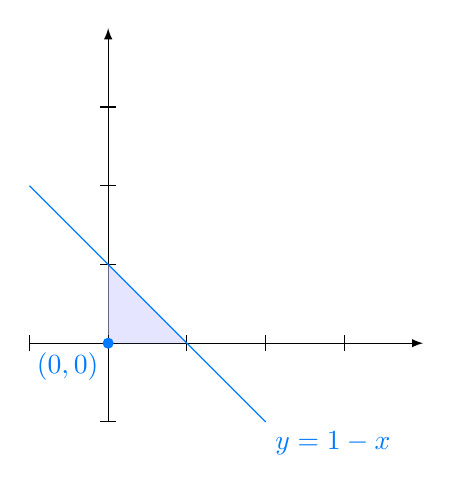
\begin{tikzpicture}[> =latex]
    \draw[->] (-1,0) -- (4,0);
    \draw[->] (0,-1) -- (0, 4);
    \node (O) at (0,0) {};
    \fill[color=blue!20, opacity=0.5]  (0,0) -- (0,1) -- (1,0) -- cycle;
    \foreach \x in {-1,...,3} {
      \draw (\x, 0.1) -- (\x, -0.1);
    }
    \foreach \y in {-1,...,3} {
      \draw (0.1, \y) -- (-0.1,\y);
    }
    \draw[lightblue, domain=-1:2] plot (\x, {1-\x}) node[below right] {$y=1-x$};
    \fill[lightblue] (O) circle (2pt) node[below left] {$(0,0)$};
  \end{tikzpicture}
\end{center}

\begin{enumerate}[label=Paso \arabic*:]
  \item Región de integración

    La región triangular está definida como: 
    \begin{itemize}[label=\textbullet]
      \item $x\ge 0$
      \item $y\ge 0$
      \item $x+y\le 1$
    \end{itemize}
    En términos de límites:
    \begin{itemize}[label=\textbullet]
      \item $x \in [0,1]$
      \item Para un valor fijo de $x,y\in [0, 1-x]$
    \end{itemize}
  \item Cambio de variable

    Observamos que el integrando involucra la expresión $\frac{x-y}{x+y}$. Esto sugiere un cambio de variables adecuado para simplificar la integración. Definimos: \[
    u=x+y,\quad v=x-y
    \] 
    Con esto:
    \begin{itemize}[label=\textbullet]
      \item $x=\dfrac{u+x}{2},\quad y=\dfrac{u-v}{2}  $
      \item El jacobiano del cambio de variables es:
        \[
        \begin{vmatrix}
          \frac{\partial x}{\partial u} & \frac{\partial x}{\partial v} \\
            \frac{\partial y}{\partial u} & \frac{\partial y}{\partial v} 
        \end{vmatrix} = \begin{vmatrix} 
            \dfrac{1}{2} & \dfrac{1}{2}\\
            \dfrac{1}{2} & -\dfrac{1}{2}
        \end{vmatrix} =\left( -\dfrac{1}{4}-\dfrac{1}{4} \right)=-\dfrac{1}{2} 
        \] 
    \end{itemize}
    Por lo tanto, $\dx \dy =\dfrac{1}{2}\du \dv $.
  \item Región en las nuevas variables

    La región $\Omega$ en las variables $(u,v)$ se transforma como sigue:
     \begin{itemize}[label=\textbullet]
       \item $x+y=u$, con  $u\in [0,1]$.
       \item $x-y=v$, con  $v\in [-u,u]$.
    \end{itemize}
    Por lo tanto, la región en $(u,v)$ está definida por:  \[
      u\in [0,1],\quad v\in [-u,v].
    \] 
  \item Reescribir la integral

    El integrando se convierte en: \[
    \dfrac{x-y}{x+y} =\dfrac{v}{u}.
    \] 
    La integral original se transforma en: \[
    \iint_{\Omega}e^{\frac{x-y}{x+y} } \dx \dy =\int_{0}^{1} \int_{-u}^{u} e^{\frac{v}{u} } \cdot \dfrac{1}{2}\dv \du .  
    \] 
  \item Resolver la integral 

    Para $u$ fijo, integramos respecto a  $v$:  \[
    \int_{-u}^{u} e^{\frac{v}{u} } \dv . 
    \] 
Realizamos el cambio de variable $t=\dfrac{v}{u}$, de donde: \[
v=ut,\quad\dv =u\dt
\] 
Los límites de integración cambian:
\begin{itemize}[label=\textbullet]
  \item Cuando $v=-u,\, t=-1$
  \item Cuando  $v=u,\, t=1$
\end{itemize}
La integral respecto a $v$ se convierte en:  \[
  \int_{-u}^{u} e^{\frac{v}{u} } \dv =\int_{-1}^{1} e^{t}\cdot u\dt=u \int_{-1}^{1} e^{t}\dt=u\cdot [e^{t} ]_{-1}^1=u\cdot \left(e-\dfrac{1}{e}\right)
\] 
Sustituimos el resultado interior en la integral original: \[
  V=\dfrac{1}{2}\int_{0}^{1} u\left( e-\dfrac{1}{e} \right) \du =\dfrac{1}{2}\left( e-\dfrac{1}{e} \right) \int_{0}^{1} u\du =\dfrac{1}{2}\left( e-\dfrac{1}{e} \right) \cdot \left[ \dfrac{u^2}{2} \right] _0^1=\bboxed{\dfrac{1}{4}\cdot \left( e-\dfrac{1}{e} \right)}
\] 
\end{enumerate}

\item \lb{Calcular el volumen comprendido entre los cilindros $z=x^{2}$ y $z=4-y^{2}$.}

  Nos piden calcular el volumen del sólido comprendido entre los cilindros parabólicos:
  \begin{enumerate}[label=\arabic*)]
    \item $z=x^2$ (abierto hacia el plano $xy$ en  $x$).
    \item $z=4-y^2$ (abierto hacia el plano $xy$ en  $y$).
  \end{enumerate}
  \begin{enumerate}[label=Paso \arabic*:]
    \item Determinar la región en el plano $xy$

      Para encontrar la región en el plano $xy$, igualamos las ecuaciones de los cilindros:  \[
      x^2=4-y^2\longrightarrow x^2+y^2=4
      \]
      Esto corresponde a un círculo de radio $2$ centrado en el origen.

      La región de proyección en el plano  $xy$ está dada por:  \[
      x^2+y^2\le 4
      \] 
    \item Expresar el volumen como una integral

      El volumen del sólido está dado por:
      \[
        V=\iint_{\text{Región}}[(z_\mathrm{sup}- z_\mathrm{inf})]\:\mathrm{d}A,
      \] 
      donde:
      \begin{itemize}[label=\textbullet]
        \item $z_\mathrm{sup}=4-y^2$ 
        \item $z_\mathrm{inf}=x^2$
      \end{itemize}
      Por lo tanto: \[
      z_\mathrm{sup} - z_\mathrm{inf} = (4-y^2)-x^2=4-x^2-y^2
      \] 
      La integral del volumen se convierte en:
      \[
      V=\iint_{x^2+y^2\le 4}(4-x^2-y^2)\:\mathrm{d}A.
      \] 
    \item Cambiar a coordenadas polares:

      En coordenadas polares:
      \begin{itemize}[label=\textbullet]
        \item $x=r\cos\theta,\, y=r\sin\theta$
        \item $x^2+y^2=r^2$ 
        \item $\:\mathrm{d}A=r\dr \dth $
      \end{itemize}
      La región se describe como: \[
        r\in [0,2],\quad\theta\in [0,2\pi].
      \] 
      El integrando se convierte en: \[
      4-x^2-y^2=4-r^2.
      \] 
      La integral en coordenadas polares es: \[
      V=\int_{0}^{2\pi} \int_{0}^{2} (4-r^2)\cdot r\dr \dth .  
      \] 
    \item Resolver la integral
\[
  \begin{array}{l} 
  \int_{0}^{2} 4r-r^3\dr =\left[2r^2-\dfrac{r^4}{4}\right]_0^2=8-4=4 \\
  \int_{0}^{2\pi} 4\dth =4\cdot [\theta]_0^{2\pi}=\bboxed{8\pi}  
  \end{array}
\] 
  \end{enumerate}

\item \lb{Calcular el volumen del balón de Rugby de ecuaciones $\dfrac{x^{2}}{a^{2}}+\dfrac{y^{2}}{b^{2}}+\dfrac{z^{2}}{c^{2}}=1$.}

Nos piden calcular el volumen del sólido definido por la ecuación: \[
\dfrac{x^2}{a^2}+\dfrac{y^2}{b^2}+\dfrac{z^2}{c^2}=1,
\] 
que describe un \textbf{elipsoide} centrado en el origen, con semiejes $a, b$, y  $c$. 
\begin{enumerate}[label=Paso \arabic*:]
  \item Reescribir la ecuación del elipsoide

    El elipsoide puede ser escrito como: \[
    x^2+y^2+z^2\le 1\quad(\text{en un espacio escalado por $a,b$ y  $c$}).
    \] 
    Para facilitar el cálculo, hacemos un cambio de variables: \[
    u=\dfrac{x}{a},\quad v=\dfrac{y}{b}, \quad w=\dfrac{z}{c}.
    \] 
    Esto transforma la ecuación del elipsoide en una esfera: \[
    u^2+v^2+w^2\le 1
    \] 
    El jacobiano del cambio de variables es: \[
    \dx \dy \dz =\det \begin{pmatrix} 
      a & 0 & 0\\
      0 & b & 0\\
      0 & 0 & c
    \end{pmatrix} \du \dv \:\mathrm{d}w=abc\du \dv \mathrm{d}w.
    \] 
    El volumen se transforma en: \[
    V=\iiint_{u^2+v^2+w^2\le 1}abc\du \dv \:\mathrm{d}w=abc \iiint_{u^2+v^2+w^2\le 1}1\du \dv \mathrm{d}w.
    \]
  \item Volumen de la esfera unitaria

    La integral restante es el volumen de una esfera unitaria en coordenadas esféricas: \[
    u=r\sin\phi\cos\theta,\quad v=r\sin\phi\sin\theta,\quad w=r\cos\phi,
    \] 
    y el elemento del volumen es: \[
    \du \dv \:\mathrm{d}w=r^2\sin\phi\dr \:\mathrm{d}\phi\dth .
    \] 
    El volumen se convierte en:
    \[
    abc\cdot \iiint_{u^2+v^2+w^2\le 1}1\du \dv \:\mathrm{d}w=abc\cdot \int_{0}^{1} \int_{0}^{\pi} \int_{0}^{2\pi}r^2\sin\phi\dth \:\mathrm{d}\phi\dr =\dfrac{1}{2}\cdot 2\cdot 2\pi\cdot abc = \bboxed{\dfrac{4\pi}{3}abc} 
    \] 
  \item Resolver las integrales

    \[
    \begin{array}{c}
      \int_{0}^{2\pi} 1\dth =[\theta]_0^{2\pi}=2\pi\\
      \int_{0}^{\pi} \sin\phi\:\mathrm{d}\phi=[-\cos\theta]_0^{2\pi}=-(-1)+1=2\\
      \int_{0}^{1} r^2\dr =\left[ \dfrac{r^3}{3} \right]_0^1=\dfrac{1}{3}  
    \end{array}
    \] 
\end{enumerate}

\item \lb{Calcular $$
\underset{\Omega}{ \iiint }\dfrac{\:\mathrm{d}x\:\mathrm{d}y\:\mathrm{d}z}{(x^{2}+y^{2}+x^{2})^{\frac{3}{2}}},
$$
donde $\Omega$ es la región limitado por las esferas $x^{2}+y^{2}+z^{2}=a^{2}$ y $x^{2}+y^{2}+z^{2}=b^{2}$, donde $0<b<a$. Indicación: hacer el cambio a coordenadas esféricas.}

Queremos calcular: \[
  \iint_\Omega \dfrac{\dx \dy \dz }{(x^2+y^2+z^2)^{\frac{2}{3} }}, 
\] 
donde $\Omega$ es la región limitada por las esferas $x^2+y^2+z^2=a^2$ y $x^2+y^2+z^2=b^2$, con $0\le b\le a$.
\begin{enumerate}[label=Paso \arabic*:]
  \item Cambio a coordenadas esféricas:
    \begin{itemize}[label=\textbullet]
      \item $x=r\sin\phi\cos\theta$
      \item $y=r\sin\phi\sin\theta$
      \item $z=r\cos\phi$ 
      \item $\dx \dy \dz =r^2\sin\phi\dr \:\mathrm{d}\phi\dth $
    \end{itemize}
    La región en coordenadas esféricas está definida por:
    \begin{itemize}[label=\textbullet]
      \item $r \in [b,a]$
      \item $\phi\in [0,\pi]$
      \item $\theta\in [0,2\pi]$
    \end{itemize}
    El integrando se transforma en: \[
      \dfrac{1}{(x^2+y^2+z^2)^{\frac{3}{2} }}=\dfrac{1}{r^3}.
    \] 
    Por lo tanto, la integral se convierte en: \[
    \iiint_\Omega\dfrac{\dx \dy \dz }{(x^2+y^2+z^2)^{\frac{3}{2} }} =\int_{0}^{2\pi} \int_{0}^{\pi} \int_{b}^{a} \dfrac{r^2\sin\phi}{r^3} \dr \:\mathrm{d}\phi\dth =\int_{0}^{2\pi} \int_{0}^{\pi} \int_{b}^{a} \dfrac{1}{r}\sin\phi\dr \:\mathrm{d}\phi\dth       
    \] 
  \item Separar la integral

    Separamos las integrales: \[
    \begin{array}{c}
      \int_{b}^{a} \dfrac{1}{r}\dr =[\ln(r)]_b^a=\ln(a)-\ln(b)=\ln\left( \dfrac{a}{b} \right) \\
      \int_{0}^{\pi} \sin\phi\:\mathrm{d}\phi=[-\cos(\phi)]_0^\pi=-(-1)+1=2\\
      \int_{0}^{2\pi} 1\dth =[\theta]_0^{2\pi}=2\pi 
    \end{array}
    \] 
  \item Multiplicar los resultados

    El volumen total es: \[
    V=2\pi\cdot 2\cdot \ln\left( \dfrac{a}{b} \right) =\bboxed{4\pi\ln\left( \dfrac{a}{b} \right) } 
    \] 
\end{enumerate}
\end{enumerate}

\begin{center}
  \noindent\rule{0.5\textwidth}{0.5pt}
\end{center}
\textbf{\Large Capítulo 2: Campos escalares y vectoriales}
\begin{enumerate}[label=\color{red}\textbf{\arabic*)}]
  \item \lb{Calcular el gradiente de los siguientes campos escalares:}
    \begin{enumerate}[label=\color{red}\textbf{\alph*)}]
      \item \db{$f(x,y,z)=e^{zyx} $}
      
      \[
          \nabla f=\left( \frac{\partial f}{\partial x} ,\frac{\partial f}{\partial y} ,\frac{\partial f}{\partial z}  \right) =(yze^{xyz},xze^{xyz},xye^{xyz}   )
          \] 
      \item \db{$f(x,y,z)=\dfrac{1}{\sqrt{x^2+y^2+z^2} } $} 
      
      $\begin{array}{l}
        \frac{\partial f}{\partial x} =-\dfrac{1}{2}\dfrac{1}{(x^2+y^2+z^2)^{\frac{3}{2}}} \cdot 2x=-\dfrac{x}{(x^2+y^2+z^2)^{\frac{3}{2} }} \\
        \frac{\partial f}{\partial y} =-\dfrac{1}{2}\dfrac{1}{(x^2+y^2+z^2)^{\frac{3}{2}}} \cdot 2y=-\dfrac{y}{(x^2+y^2+z^2)^{\frac{3}{2} }} \\
        \frac{\partial f}{\partial z} =-\dfrac{1}{2}\dfrac{1}{(x^2+y^2+z^2)^{\frac{3}{2}}} \cdot 2z=-\dfrac{z}{(x^2+y^2+z^2)^{\frac{3}{2} }} 
      \end{array}$

      \[
        \nabla f=\left( \frac{\partial f}{\partial }, \frac{\partial f}{\partial y} ,\frac{\partial f}{\partial z}   \right) =\left(-\dfrac{x}{(x^2+y^2+z^2)^{\frac{3}{2} }},-\dfrac{y}{(x^2+y^2+z^2)^{\frac{3}{2} }},-\dfrac{z}{(x^2+y^2+z^2)^{\frac{3}{2} }}\right) 
          \] 
      \item \db{$f(x,y,z)=\sin(xyz)$} 
        \[
        \nabla f=\left( \frac{\partial f}{\partial x} ,\frac{\partial f}{\partial y} ,\frac{\partial f}{\partial z}  \right) =\left( \cos(xyz)\cdot yz,\cos(xyz)\cdot xz,\cos(xyz)\cdot xy \right) 
        \] 
      \item \db{$\cos(x+y+z)$} 
        \[
        \nabla f=\left( \frac{\partial f}{\partial x} ,\frac{\partial f}{\partial y} ,\frac{\partial f}{\partial z} \right) =(-\sin(x+y+z), -\sin(x+y+z), -\sin(x+y+z))
        \] 
    \end{enumerate}
  \item \lb{Calcular la divergencia y el rotacional de los siguientes campos:}

    Vamos a calcular la \textbf{divergencia} y el \textbf{rotacional}. Las fórmulas son: 
\begin{enumerate}[label=\arabic*)]
  \item \textbf{Divergencia} de $\mathbf{F}=F_x\mathbf{i} +F_y\mathbf{j} +F_z\mathbf{k}:$ 
    \[
    \nabla \cdot \mathbf{F} =\frac{\partial F_x}{\partial x} +\frac{\partial F_y}{\partial y} +\frac{\partial F_z}{\partial z} 
    \] 
  \item \textbf{Rotacional} de $\mathbf{F} =F_x\mathbf{i} +F_y\mathbf{j} +F_z\mathbf{k} $:
    \[
    \nabla \times \mathbf{F} =\begin{vmatrix} 
      \mathbf{i}  & \mathbf{j} & \mathbf{k} \\
      \frac{\partial }{\partial x} & \frac{\partial }{\partial y} & \frac{\partial }{\partial z} \\
      F_x & F_y & F_z
    \end{vmatrix}. 
    \] 
\end{enumerate}
    \begin{enumerate}[label=\color{red}\textbf{\alph*)}]
      \item \db{$\mathbf{F}(x,y,z)=(\sin x)\mathbf{i}+(\cos)\mathrm{j}$.} 
        \begin{enumerate}[label=\arabic*)]
          \item Divergencia:
            \[
              \nabla \cdot \mathbf{F} =\frac{\partial (\sin x)}{\partial x} +\frac{\partial (\cos x)}{\partial y} +\frac{\partial (0)}{\partial z} = \cos x+0+0=\cos x
            \] 
          \item Rotacional:
            \[
            \nabla \times \mathbf{F} = \begin{vmatrix} 
              \mathbf{i}  & \mathbf{j} & \mathbf{k} \\
              \frac{\partial }{\partial x} & \frac{\partial }{\partial y} & \frac{\partial V}{\partial z} \\
              \sin x & \cos x & 0
            \end{vmatrix} =\mathbf{i} (0,0)-\mathbf{j} (0-0)+\mathbf{k} \left( \frac{\partial (\cos x)}{\partial x} -\frac{\partial (\sin )}{\partial y}  \right) =\mathbf{k} (-\sin x-0)=-\sin x\mathbf{k} 
            \] 
        \end{enumerate}
      \item \db{$\mathbf{F}(x,y,z)=x\mathbf{i}-y\mathbf{j}$.} 
        \begin{enumerate}[label=\arabic*)]
          \item Divergencia
            \[
            \nabla \cdot \mathbf{F} =\frac{\partial (x)}{\partial x} +\frac{\partial (-y)}{\partial y} +\frac{\partial 0}{\partial z} =1-1+0=0
            \] 
          \item Rotacional
            \[
            \nabla \times \mathbf{F} =\begin{vmatrix} 
              \mathbf{i} & \mathbf{j}  & \mathbf{k} \\
              \frac{\partial }{\partial x} & \frac{\partial }{\partial y} & \frac{\partial }{\partial z} \\
              x & -y & 0
          \end{vmatrix}=\mathbf{i} (0-0)-\mathbf{j} (0-0)+\mathbf{j} \left( \frac{\partial (-y)}{\partial x} -\frac{\partial (x)}{\partial y}  \right) = 0
            \] 
        \end{enumerate}
      \item \db{$\mathbf{F}(x,y,z)=ax\mathbf{i}+by\mathbf{j}-^3fk$, donde $a,b,c\in \R$.} 
      \begin{enumerate}[label=\arabic*)]
                \item Divergencia
                  \[
                  \nabla \cdot \mathbf{F} =\frac{\partial (ax)}{\partial x} +\frac{\partial (by)}{\partial y} +\frac{\partial (-cz)}{\partial z} =a+b-c
                  \] 
                \item Rotacional
                  \[
                  \nabla \times \mathbf{F} =\begin{vmatrix} 
                    \mathbf{i}  & \mathbf{j} & \mathbf{k} \\
                    \frac{\partial }{\partial x} & \frac{\partial }{\partial y} & \frac{\partial }{\partial z} \\
                    ax & by & -cz
                  \end{vmatrix}=\mathbf{i} (0-0)-\mathbf{j} (0-0)+\mathbf{k} (0-0)=0 
                  \] 
              \end{enumerate}
      \item \db{$\mathbf{F}(x,y,z)=x^2\mathbf{i}+y^2\mathbf{j}-z^2\mathbf{k}$.} 
      \begin{enumerate}[label=\arabic*)]
                \item Divergencia
                  \[
                  \nabla \cdot \mathbf{F} =\frac{\partial (x^2)}{\partial x}+\frac{\partial (y^2)}{\partial y} +\frac{\partial (-z^2)}{\partial z}=2x+2y-2z
                  \] 
                \item Rotacional
                  \[
                  \nabla \times \mathbf{F} =\begin{vmatrix} 
                    \mathbf{i}  & \mathbf{j} &\mathbf{k} \\
                    \frac{\partial }{\partial x} & \frac{\partial }{\partial y} & \frac{\partial }{\partial z} \\
                    x^2 & y^2 & -z^2
                  \end{vmatrix} =\mathbf{i} (0-0)-\mathbf{j} (0-0)+\mathbf{k} (0-0)=0
                  \] 
              \end{enumerate}
      \item \db{$\mathbf{F}(x,y,z)=xy\mathbf{i}+yz\mathbf{j}+xz\mathbf{k}$.} 
        \begin{enumerate}[label=\arabic*)]
          \item Divergencia:
            \[
            \nabla \cdot \mathbf{F} =\frac{\partial (xy)}{\partial x} +\frac{\partial (yz)}{\partial y} +\frac{\partial (xz)}{\partial z} =y+z+x
            \] 
          \item Relacional:
            \[
            \nabla \times \mathbf{F} =\begin{vmatrix} 
              \mathbf{i} & \mathbf{j} & \mathbf{k} \\
              \frac{\partial }{\partial x} & \frac{\partial }{\partial y} & \frac{\partial }{\partial z} \\
              xy & yz & xz
            \end{vmatrix} =\mathbf{i} (z-z)-\mathbf{j} (x-x)+\mathbf{k} (y-y)=0
            \] 
        \end{enumerate}
      \item \db{$\mathbf{F}(x,y,z)=xyz\mathbf{i}+x^2y^2z^2\mathbf{j}+y^2z^3\mathbf{k}$.} 
      \begin{enumerate}[label=\arabic*)]
                \item Divergencia:
                  \[
                  \nabla \cdot F = \frac{\partial (xyz)}{\partial x} +\frac{\partial (x^2y^2z^2)}{\partial y} +\frac{\partial (y^2z^3)}{\partial z} =yz+2x^2yz^2+3y^2z^2
                  \] 
                \item Relacional:
                  \[
                  \begin{aligned}
                  \nabla \times \mathbf{F} =\begin{vmatrix} 
                    \mathbf{i}  & \mathbf{j} & \mathbf{k} \\
                    \frac{\partial }{\partial x} & \frac{\partial }{\partial y}  & \frac{\partial }{\partial z} \\
                    xyz & x^2y^2z^2 & y^2z^3
                  \end{vmatrix} &= \mathbf{i} (2xz^3-2x^2y^2z)-\mathbf{j} (xy-0)+\mathbf{k} (2xy^2z^2-xz)\\
                  &=(2xz^3-2x^2y^2z)\mathbf{i} -xy\mathbf{j} +(2xy^2z^2-xz)\mathbf{k} 
                  \end{aligned}
                  \] 
              \end{enumerate}
    \end{enumerate}
  \item \lb{Sea $f\in C^2(D,\R)$. Se define el \textit{Laplaciano de $f$} como la divergencia del gradiente de $f$, esto es  \[
  \nabla^2f= <\nabla,\nabla f > = \mathrm{div}(\nabla f).
  \] 
Una función $f$ se dice  \textit{armónica} si $\nabla ^2f=0$. Identificar cuáles de las siguientes funciones son armónicas:}
\begin{enumerate}[label=\color{red}\textbf{\alph*)}]
  \item \db{$f(x,y)=e^{z}\cos y$.}

    \[
    \nabla ^2f=\frac{\partial^2 f}{\partial x^2} +\frac{\partial^2 f}{\partial y^2} +\frac{\partial^2 f}{\partial z^2} = 0 + (-e^{z}\cos y )+e^{z}\cos y=0\longrightarrow f(x,y,z)\text{ es armónica} 
    \] 
    
    $\begin{array}{l}
      \frac{\partial f}{\partial x} = 0\longrightarrow \frac{\partial^2 f}{\partial x^2} =0\\
      \frac{\partial f}{\partial y} =e^{z}(-\sin y)\longrightarrow \frac{\partial^2 f}{\partial y^2} =e^{z}(-\cos y)  \\
      \frac{\partial f}{\partial z} =e^{z}\cos y\longrightarrow \frac{\partial^2 f}{\partial z^2} =e^{z} \cos y 
    \end{array}$
  \item \db{$f(x,y,z)=e^{-z}(\cos y-\sin y) $.}
    
    \[
    \nabla ^2f=\frac{\partial^2 f}{\partial x^2} +\frac{\partial^2 f}{\partial y^2} +\frac{\partial^2 f}{\partial z^2} = 0 + e^{-z}(-\cos y+\sin y)+e^{-z}(\cos y -\sin y)=0\longrightarrow f(x,y,z)\text{ es armónica }  
    \] 

    $\begin{array}{l}
      \frac{\partial f}{\partial x} =0\longrightarrow \frac{\partial^2 f}{\partial x^2} =0\\
      \frac{\partial f}{\partial y} =e^{-z}(-\sin y-\cos y)\longrightarrow \frac{\partial^2 f}{\partial y^2} e^{-z}(-\cos y + \sin y)\\
      \frac{\partial f}{\partial z} =e^{-z}(-\cos y + \sin y)\longrightarrow \frac{\partial^2 f}{\partial z^2} =e^{-z}(\cos y -\sin y)  
    \end{array}$
  \item \db{$f(x,y,z)=(x^2+y^2+z^2)^{-\frac{1}{2} }$.} 

    \[
      \begin{aligned}
      \nabla ^2f=\frac{\partial^2 f}{\partial x^2} +\frac{\partial^2 f}{\partial y^2} +\frac{\partial^2 f}{\partial z^2} &=  3x^2(x^2+y^2+z^2)^{-\frac{5}{2} }+3y^2(x^2+y^2+z^2)^{-\frac{5}{2} }+3z^2-3(x^2+y^2+z^2)^{-\frac{3}{2} }\neq 0\\
      & \longrightarrow f(x,y,z) \text{ no es armónica}
      \end{aligned}
    \] 
    $\begin{array}{l}
      \frac{\partial f}{\partial x} =-\dfrac{1}{2}(x^2+y^2+z^2)^{-\frac{3}{2} }\cdot 2x=-x(x^2+y^2+z^2)^{-\frac{3}{2} }\longrightarrow \frac{\partial^2 f}{\partial x^2} = -(x^2+y^2+z^2)^{-\frac{3}{2} }+3x^2(x^2+y^2+z^2)^{-\frac{5}{2} }\\
      \frac{\partial f}{\partial y} =-\dfrac{1}{2}(x^2+y^2+z^2)^{-\frac{3}{2} }\cdot 2y=-y(x^2+y^2+z^2)^{-\frac{3}{2} }\longrightarrow \frac{\partial^2 f}{\partial y^2} = -(x^2+y^2+z^2)^{-\frac{3}{2} }+3y^2(x^2+y^2+z^2)^{-\frac{5}{2} }\\
      \frac{\partial f}{\partial z} =-\dfrac{1}{2}(x^2+y^2+z^2)^{-\frac{3}{2} }\cdot 2z=-z(x^2+y^2+z^2)^{-\frac{3}{2} }\longrightarrow \frac{\partial^2 f}{\partial z^2} = -(x^2+y^2+z^2)^{-\frac{3}{2} }+z^2(x^2+y^2+z^2)^{-\frac{5}{2} }\\
    \end{array}$
\end{enumerate}
\item \lb{Dadas las funciones $\mathbf{F}(x,y,z)=2\mathrm{i}+2x\mathbf{j}+3y\mathbf{k}$ y $\mathbf{G}(x,y,z)=x\mathbf{i}-y\mathbf{j}+z\mathbf{k}$, calcular:}
  \begin{enumerate}[label=\color{red}\textbf{\alph*)}]
    \item \db{$\mathrm{rot}(\mathbf{F}\times \mathbf{G})$} 

      La fórmula del rotaciona del producto vectorial de dos campos $\mathbf{F} $ y $\mathbf{G} $ es: \[
      \mathrm{rot} (\mathbf{F} \times \mathbf{G} )=(\mathbf{G} \cdot \nabla)\mathbf{F} -(\mathbf{F} \cdot \nabla )\mathbf{G} +F(\nabla \cdot \mathbf{G} )-\mathbf{G} (\nabla \cdot \mathbf{F} )
      \] 
      \begin{enumerate}[label=Paso \arabic*:]
        \item Calcular $\nabla \cdot \mathbf{F} $ y $\nabla \cdot \mathbf{G} $ 
          \begin{itemize}[label=\textbullet]
            \item $\mathbf{F} (x,y,z)=2\mathbf{i} +2x\mathbf{j} +3y\mathbf{k} $: \[
            \nabla \cdot \mathbf{F} =\frac{\partial (2)}{\partial x} +\frac{\partial (2x)}{\partial y} +\frac{\partial (3y)}{\partial z} =0
            \] 
          \item $\mathbf{G} (x,y,z)=x\mathbf{i} -y\mathbf{j} +z\mathbf{k} $: \[
          \nabla \cdot \mathbf{G} =\frac{\partial (x)}{\partial x} +\frac{\partial (-y)}{\partial z} +\frac{\partial (z)}{\partial z} =1-1+1=1
          \] 
          \end{itemize}
      \item Calcular $(\mathbf{G} \cdot \nabla )\mathbf{F} $ y $(\mathbf{F} \cdot \nabla )\mathbf{F} $
        \begin{itemize}[label=\textbullet]
          \item Para $(\mathbf{G} \cdot \nabla )\mathbf{F}$: \[
          G\cdot \nabla =x \frac{\partial }{\partial x} -y \frac{\partial }{\partial y} +z \frac{\partial }{\partial z} .
          \] 
          Aplicamos este operacdor a cada componente de $\mathbf{F} $:
          \[
          \begin{array}{c}
            (\mathbf{F} \cdot \nabla)\mathbf{F}_x=x\cdot \frac{\partial (2)}{\partial x} -y\cdot \frac{\partial (2)}{\partial y} +z\cdot \frac{\partial (2)}{\partial z} =0\\
            (\mathbf{G} \cdot \nabla )\mathbf{F} _y=x\cdot \frac{\partial (2x)}{\partial x} -y\cdot \frac{\partial (2x)}{\partial y} +z\cdot \frac{\partial (2x)}{\partial z} =2x\\
            (G\cdot \nabla )\mathbf{F} _z=x\cdot \frac{\partial (3y)}{\partial x} -y\cdot \frac{\partial (3y)}{\partial y} +z\cdot \frac{\partial (3y)}{\partial z} =-3y\\
            (\mathbf{G} \cdot \nabla )\mathbf{F} =O\mathbf{i} +2x\mathbf{j} -3y\mathbf{k} 
          \end{array}
          \] 
        \item Para $(\mathbf{F} \cdot \nabla )\mathbf{G}$:
          \[
          \mathbf{F} \cdot \nabla =2 \frac{\partial }{\partial x} +2x \frac{\partial }{\partial y} +3y \frac{\partial }{\partial z} .
          \]
          Aplicamos este operador a cada componente de $\mathbf{G} $:
          \[
          \begin{array}{c}
            (\mathbf{F} \cdot \nabla )\mathbf{G} _x=2\cdot \frac{\partial (x)}{\partial x} +2x\cdot \frac{\partial (x)}{\partial y} +3y\cdot \frac{\partial (x)}{\partial z} =2\\
            (\mathbf{F} \cdot \nabla )\mathbf{G} _y=2\cdot \frac{\partial (-y)}{\partial x} +2x\cdot \frac{\partial (-y)}{\partial y} +3y\cdot \frac{\partial (-y)}{\partial z} =-2y\\
            (\mathbf{F} \cdot \nabla )\mathbf{G} _z=2\cdot \frac{\partial (z)}{\partial x} +2x\cdot \frac{\partial (z)}{\partial x} +3y\cdot \frac{\partial (z)}{\partial z} =3y\\
            (\mathbf{F} \cdot \nabla )\mathbf{G} =2\mathbf{i} -2x\mathbf{j} +3y\mathbf{k} 
          \end{array}
          \] 
        \end{itemize}
      \item Sustituir en la fórmula \[
      \mathrm{rot} (\mathbf{F} \times \mathbf{G} )=(\mathbf{G} \cdot \nabla )\mathbf{F} -(\mathbf{F} \cdot \nabla)\mathbf{G} +\mathbf{F} (\nabla \cdot G)-\mathbf{G} (\nabla \cdot F)
      \] 
      \begin{enumerate}[label=\arabic*)]
        \item $(\mathbf{G} \cdot \nabla)\mathbf{F} -(F\cdot \nabla )\mathbf{G}=(0\mathbf{i} +2x\mathbf{j}-3y\mathbf{k}  )-(2\mathbf{i} -2x\mathbf{j} +3y\mathbf{k} )=-2\mathbf{i} +4x\mathbf{j} -4y\mathbf{k} $
      \item $\mathbf{F} (\nabla \cdot \mathbf{G} )=1\cdot F=2\mathbf{i} +2x\mathbf{j} +3y\mathbf{k} $
      \item $-\mathbf{G} (\nabla \cdot \mathbf{F} )=-2(x\mathbf{i} -y\mathbf{j} +z\mathbf{k} )=-2\mathbf{i} +2y\mathbf{j}-2z\mathbf{k}$
      \end{enumerate}
      Sumamos todas las contribuciones:
      \[
      \mathrm{rot} (\mathbf{F} \times \mathbf{G} )=(-2+2-2x)\mathbf{i} +(4x+2x+2y)\mathbf{j} +(-yy+3y-2z)\mathbf{k} =(-2x)\mathbf{i} +(6x+2y)\mathbf{j} +(-3y-2z)\mathbf{k} .
      \] 
      \end{enumerate}
    \item \db{$\mathrm{div}(\mathbf{F}\times \mathbf{G})$} 
      \begin{enumerate}[label=Paso \arabic*:]
        \item Calcular $\mathbf{F} \times \mathbf{G} $

          El producto cruzado es: \[
          \begin{aligned}
          \mathbf{F} \times \mathbf{G} =\begin{vmatrix} 
            \mathbf{i}  & \mathbf{j} &\mathbf{k} \\
            2 & 2x & 3y\\
            x & -y & z
          \end{vmatrix}=\mathbf{i} \begin{vmatrix} 
            2x & 3y\\
            -y & z
          \end{vmatrix} -\mathbf{j} \begin{vmatrix} 
            2 & 3y\\
            x & z
          \end{vmatrix}  +\mathbf{k} \begin{vmatrix} 
            2 & 2x\\
            x & -y
          \end{vmatrix} &=\mathbf{i} (2x\cdot z-3y\cdot (-y)-\mathbf{j} (2z-3xy))+\mathbf{k} (-2y-2x^2)\\
          &=(2xz+3y^2)\mathbf{i} -(2z-3xy)\mathbf{j} +(-2y-x^2)\mathbf{k}
          \end{aligned}
          \] 
        \item Calcular $\mathrm{div} (\mathbf{F} \times \mathbf{G} )$

          La divergencia es:
          \[
          \mathrm{div} (\mathbf{F} \times \mathbf{G} )=\frac{\partial }{\partial x} (2xz+3y^2)+\frac{\partial }{\partial y} (-(2z-3xy))+\frac{\partial }{\partial z} (-2y-2x^2)=2z+3x+0=2x+3x
          \] 
      \end{enumerate}
  \end{enumerate}

\item \lb{Sean $f$ y  $g$ dos campos escalares,  $\mathbf{F}$ y $\mathbf{G}$ dos campos vectoriales y,  $\alpha\in \R$. Demostrar las siguientes propiedades:} 
  \begin{enumerate}[label=\color{red}\textbf{\alph*)}]
    \item \db{$\nabla (\alpha f)=\alpha\nabla (f)$.} 

      \[
        \nabla (\alpha f)=\left( \frac{\partial (\alpha f)}{\partial x} ,\frac{\partial (\alpha f)}{\partial y},\frac{\partial (\alpha f)}{\partial z}   \right) =\left(\alpha \frac{\partial f}{\partial x} ,\alpha \frac{\partial f}{\partial y} ,\alpha \frac{\partial f}{\partial z}\right)=\alpha \left( \frac{\partial f}{\partial x} ,\frac{\partial f}{\partial y} ,\frac{\partial f}{\partial z}  \right) =\alpha \nabla (f)
      \] 
    \item \db{$\nabla (f+g)=\nabla (f)+\nabla (g)$} 

      \[
      \nabla (f+g)=\left( \frac{\partial (f+g)}{\partial x},\frac{\partial (f+g)}{\partial y} ,\frac{\partial (f+g)}{\partial z}  \right) =\left( \frac{\partial f}{\partial x} +\frac{\partial g}{\partial x} ,\frac{\partial f}{\partial y} +\frac{\partial g}{\partial y},\frac{\partial f}{\partial z}+\frac{\partial g}{\partial z}   \right) =\left( \frac{\partial f}{\partial x} ,\frac{\partial f}{\partial y} ,\frac{\partial f}{\partial z}  \right) +\left( \frac{\partial g}{\partial x} ,\frac{\partial g}{\partial y} ,\frac{\partial g}{\partial z}  \right)
    \]
    Por lo tanto: \[
    \nabla (f+g) =\nabla (f)+\nabla (g)
    \] 
    \item \db{$\nabla \left( \dfrac{f}{g} \right) =\dfrac{g\nabla (f)-f\nabla (g)}{g^2},\,g\neq 0$.}
    \[
    \nabla \left( \dfrac{f}{g} \right) =\left( \dfrac{\frac{\partial f}{\partial x} g-f \frac{\partial g}{\partial x} }{g^2},\dfrac{\frac{\partial f}{\partial y} g-f \frac{\partial h}{\partial y} }{g^2},\dfrac{\frac{\partial f}{\partial z} g-f \frac{\partial g}{\partial z} }{g^2}   \right) =\dfrac{g\nabla (f)-f\nabla (g)}{g^2} 
    \] 
    \item \db{$\nabla (fg)=f\nabla g+g\nabla (f)$}
      
      \[
      \nabla (fg)=\left( \frac{\partial f}{\partial x} g+f \frac{\partial g}{\partial x} ,\frac{\partial f}{\partial y} g+f \frac{\partial g}{\partial y} ,\frac{\partial f}{\partial z} g+f \frac{\partial g}{\partial z}  \right) =f\nabla (g)+g\nabla (f)
      \] 
    \item \db{$\mathrm{div}(\alpha\mathbf{F})=\alpha\mathrm{div}(\mathbf{F})$.} 

      \[
      \begin{array}{l}
        \alpha \mathbf{F} =\alpha F_x\mathbf{i} +\alpha F_y\mathbf{j} +\alpha F_z\mathbf{k}\\ 
        \mathrm{div} (\alpha \mathbf{F} )=\nabla \cdot (\alpha \mathbf{F} )=\frac{\partial (\alpha F_x)}{\partial x} +\frac{\partial (\alpha F_y)}{\partial y} +\frac{\partial (\alpha F_z)}{\partial z}=\alpha \frac{\partial F_x}{\partial x} + \alpha \frac{\partial F_y}{\partial y} +\alpha \frac{\partial F_z}{\partial z}=\alpha\left( \frac{\partial F_x}{\partial x} +\frac{\partial F_y}{\partial y} +\frac{\partial F_z}{\partial z}  \right) =\alpha \mathrm{div} (\mathbf{F} ) \\
      \end{array}
      \] 
    \item \db{$\mathrm{div}(\mathbf{F}+\mathbf{G})=\mathrm{div}(\mathbf{F})+\mathrm{div}(\mathbf{G})$.} 
      \[
      \begin{array}{l}
        \mathbf{F} +\mathbf{G} =(F_x+G_x)\mathbf{i} +(F_y+G_y)\mathbf{j} +(F_z+G_z)\mathbf{k} \\
        \begin{aligned}
        \mathrm{div} (\mathbf{F} +\mathbf{G} )=\nabla \cdot (\mathbf{F} +\mathbf{G} )&=\frac{\partial (F_x+G_x)}{\partial x} +\frac{\partial (F_y+G_y)}{\partial y} +\frac{\partial (F_z+G_z)}{\partial z} =\frac{\partial F_x}{\partial x}+\frac{\partial G_x}{\partial x} +\frac{\partial F_y}{\partial y} +\frac{\partial G_y}{\partial y} +\frac{\partial F_z}{\partial z} +\frac{\partial G_z}{\partial z}   \\
        &=\left(\frac{\partial F_x}{\partial x}+\frac{\partial F_y}{\partial y}+\frac{\partial F_z}{\partial z} \right)+\left( \frac{\partial G_x}{\partial x}+\frac{\partial G_y}{\partial y} +\frac{\partial G_z}{\partial z}   \right) =\mathrm{div} (\mathbf{F} )+\mathrm{div} (\mathbf{G} )
        \end{aligned}
      \end{array}
      \] 
    \item \db{$\mathrm{rot}(\mathbf{F}+\mathbf{G})=\mathrm{rot}(\mathbf{F})+\mathrm{rot}(\mathbf{G})$.} 

      \[
      \mathrm{rot} (\mathbf{F} +\mathbf{G} )=\nabla \times (\mathbf{F} +\mathbf{G} )=(\nabla\times  \mathbf{F} )+(\nabla \times \mathbf{G} )=\mathrm{rot} (\mathbf{F} )+\mathrm{rot} (\mathbf{G} )
      \] 
    \item \db{$\mathrm{rot}(\alpha\mathbf{F})=\alpha\mathrm{rot}(\mathbf{F})$} 
      \[
      \mathrm{rot} (\alpha \mathbf{F} )=\nabla \times (\alpha\mathbf{F} )=\alpha(\nabla \times \mathbf{F} )=\alpha\mathrm{rot} (\mathbf{F} )
      \] 
    \item \db{$\mathrm{div}(\mathbf{F}\times \mathbf{G})= <\mathrm{rot}(\mathbf{F}), \mathbf{G} > - <\mathbf{F},\mathrm{rot}(G) >$} 

      Sea $\mathbf{F} \times \mathbf{G} =\mathbf{H}=H_x\mathbf{i} +H_y\mathbf{j} +H_z\mathbf{k} $, donde: \[
      \begin{array}{c}
      \mathbf{F} \times \mathbf{G} =\begin{vmatrix} 
        \mathbf{i}  & \mathbf{j}  & \mathbf{k} \\
        F_x & F_y & F_z\\
        G_x & G_y & G_z
      \end{vmatrix}\\
      H_x=F_yG_z-F_zG_y,\quad H_y=F_zG_x-F_xG_z,\quad H_z=F_xG_y-F_yG_x.
      \end{array}
      \] 
      La divergencia de $\mathbf{H}$ es:
      \[
      \mathrm{div} (\mathbf{H})=\frac{\partial H_x}{\partial x} +\frac{\partial H_y}{\partial y} +\frac{\partial H_z}{\partial z} .
      \] 
      Susituimos cada cmponente $H_x,H_y,H_z$ y derivamos:
       \[
      \begin{array}{l}
        \frac{\partial H_x}{\partial x} =\frac{\partial (F_yG_z)}{\partial x} -\frac{\partial (F_zG_y)}{\partial x} =\left( \frac{\partial F_y}{\partial x} G_z+F_y \frac{\partial G_z}{\partial x}  \right) - \left( \frac{\partial F_z}{\partial x} G_y+F_z \frac{\partial G_y}{\partial x}  \right)\\
        \frac{\partial H_y}{\partial y} =\frac{\partial (F_zG_x)}{\partial y} -\frac{\partial (F_xG_z)}{\partial y} =\left( \frac{\partial F_z}{\partial y} G_x+F_z \frac{\partial G_x}{\partial y}  \right) -\left( \frac{\partial F_x}{\partial y} G_z+F_x \frac{\partial G_z}{\partial y}  \right) \\
        \frac{\partial H_z}{\partial z} =\frac{\partial (F_xG_y)}{\partial z} -\frac{\partial (F_yG_x)}{\partial z} =\left( \frac{\partial F_x}{\partial z} G_y+F_x \frac{\partial G_y}{\partial z}  \right) - \left( \frac{\partial F_y}{\partial z} G_x+F_y \frac{\partial G_x}{\partial z}  \right)
      \end{array}
      \] 
      Sumamos todos los términos:
      \[
      \begin{aligned}
      \mathrm{div} (\mathbf{F} \times \mathbf{G} )=&G_z\left( \frac{\partial F_y}{\partial x}-\frac{\partial F_x}{\partial y}   \right) +G_x\left( \frac{\partial F_z}{\partial y} -\frac{\partial F_y}{\partial z}  \right) +G_y\left( \frac{\partial F_x}{\partial z} -\frac{\partial F_z}{\partial x}  \right)\\
      & -F_z\left( \frac{\partial G_y}{\partial x} -\frac{\partial G_x}{\partial y}  \right) -F_x\left( \frac{\partial G_z}{\partial y} -\frac{\partial G_y}{\partial z}  \right) -F_y\left( \frac{\partial G_x}{\partial z} -\frac{\partial G_z}{\partial x}  \right) =\left<\mathrm{rot} (\mathbf{F} ),\mathbf{G}  \right>-\left<\mathbf{F} ,\mathrm{rot} (\mathbf{G} ) \right>
      \end{aligned}
      \] 
    \item \db{$\mathrm{rot}(f\mathbf{F})=f\mathrm{rot}(\mathbf{F})+(\nabla f\times \mathbf{F})$}
      \[
      \mathrm{rot} (f\mathbf{F} )=\nabla \times (f\mathbf{F} )=f(\nabla \times F)+(\nabla f\times \mathbf{F} )=f\mathrm{rot} (\mathbf{F} )+(\nabla f\times \mathbf{F} )
      \] 
    \item \db{$\mathrm{div}(f\mathbf{F})=f\mathrm{div}(\mathbf{F})+<\nabla f,\mathbf{F} >$} 

      \[
      \mathrm{div} (f\mathbf{F} )=\nabla \cdot (f\mathbf{F} )=f(\nabla \cdot \mathbf{F} )+\left<\nabla f, \mathbf{F}  \right> = f\mathrm{div} (\mathbf{F} )+\left< \nabla f,\mathbf{F}  \right>.
      \] 

    \item \db{$\mathrm{div}(f\nabla g)=f\mathrm{div}(\nabla g)+ <\nabla f,\nabla g >$} 
      \[
      \mathrm{div} (f\nabla g)=f(\nabla \cdot \nabla g)+\left<\nabla f,\nabla g \right> =f\nabla ^2g+\left<\nabla f, \nabla g \right>
      \] 
  \end{enumerate}

\item \lb{Determinar si los siguientes campos vectoriales son conservativos y en caso de serlo obtener su función potencial:}
  \begin{enumerate}[label=\color{red}\textbf{\alph*)}]
    \item \db{$\mathbf{F} (x,y,z)=\dfrac{2x}{x^2+y^2+z^2}\mathbf{i} +\dfrac{2y}{x^2+y^2+z^2}\mathbf{j} +\dfrac{2z}{x^2+y^2+z^2}\mathbf{k}$.} 

      El rotacional se define como: \[
      \mathrm{rot} (\mathbf{F} )=\nabla \times \mathbf{F} =\begin{vmatrix} 
        \mathbf{i}  & \mathbf{j}  & \mathbf{k} \\
        \frac{\partial }{\partial x} & \frac{\partial }{\partial y} & \frac{\partial }{\partial z} \\
        F_x & F_y & F_z
      \end{vmatrix}, 
      \] 
      donde: \[
      F_x=\dfrac{2x}{x^2+y^2+z^2},\quad F_y=\dfrac{2y}{x^2+y^2+z^2},\quad F_z=\dfrac{2z}{x^2+y^2+z^2}.   
      \] 
      \begin{enumerate}[label=\arabic*)]
        \item Primera componente en $\mathbf{i} $: \[
        \left( \frac{\partial F_z}{\partial y} -\frac{\partial F_y}{\partial z}  \right)=-\dfrac{4yz}{(x^2+y^2+z^2)^2}-\left( -\dfrac{4yz}{(x^2+y^2+z^2)^2}  \right)  =0
        \] 
        $\begin{array}{l}
          \frac{\partial F_z}{\partial y} =\frac{\partial }{\partial y} \left( \dfrac{2z}{x^2+y^2+z^2} \right) =2z\cdot \frac{\partial }{\partial y} \left( \dfrac{1}{x^2+y^2+z^2} \right) =2z\cdot\left( -\dfrac{2y}{(x^2+y^2+z^2)^2}  \right) = -\dfrac{4yz}{(x^2+y^2+z^2)^2}\\
          \frac{\partial F_y}{\partial z} =\frac{\partial }{\partial z} \left( \dfrac{2y}{x^2+y^2+z^2} \right) =2y\cdot \frac{\partial }{\partial z} \left( \dfrac{1}{x^2+y^2+z^2} \right) =2y\cdot \left( -\dfrac{2z}{(x^2+y^2+z^2)^2}  \right) =-\dfrac{4yz}{(x^2+y^2+z^2)} 
        \end{array}$
      \item Segunda componente en $\mathbf{j} $:
        \[
        \left( \frac{\partial F_x}{\partial z}-\frac{\partial F_z}{\partial x}   \right) =-\dfrac{4xz}{(x^2+y^2+z^2)^2}-\left( -\dfrac{4xz}{(x^2+y^2+z^2)^2}  \right) =0
        \] 
        $\begin{array}{l}
          \frac{\partial F_x}{\partial z} =\frac{\partial }{\partial z} \left( \dfrac{2x}{x^2+y^2+z^2} \right) =2x\cdot \frac{\partial }{\partial z} \left( \dfrac{1}{x^2+y^2+z^2} \right) =2x\cdot \left( -\dfrac{2z}{(x^2+y^2+z^2)^2} \right) =-\dfrac{4xz}{(x^2+y^2+z^2)^2}. \\
          \frac{\partial F_z}{\partial x} =\frac{\partial }{\partial x} \left( \dfrac{2z}{x^2+y^2+z^2} \right) =2z\cdot \frac{\partial }{\partial x} \left( \dfrac{1}{x^2+y^2+z^2} \right) =2z\cdot \left( -\dfrac{2x}{(x^2+y^2+z^2)^2} \right) =-\dfrac{4xz}{(x^2+y^2+z^2)^2}. 
        \end{array}$
      \item Tercera componente en $\mathbf{k} $:
        \[
        \left( \frac{\partial F_y}{\partial x} -\frac{\partial F_x}{\partial y}  \right) =-\dfrac{4xy}{(x^2+y^2+z^2)}-\left( -\dfrac{4xy}{(x^2+y^2+z^2)^2}  \right) =0
        \] 
        $\begin{array}{l}
                  \frac{\partial F_y}{\partial x} =\frac{\partial }{\partial x} \left( \dfrac{2y}{x^2+y^2+z^2} \right) =2y\cdot \frac{\partial }{\partial x} \left( \dfrac{1}{x^2+y^2+z^2} \right) =2y\cdot \left( -\dfrac{2x}{(x^2+y^2+z^2)^2} \right) =-\dfrac{4xy}{(x^2+y^2+z^2)^2}. \\
                  \frac{\partial F_x}{\partial y} =\frac{\partial }{\partial x} \left( \dfrac{2x}{x^2+y^2+z^2} \right) =2x\cdot \frac{\partial }{\partial y} \left( \dfrac{1}{x^2+y^2+z^2} \right) =2x\cdot \left( -\dfrac{2y}{(x^2+y^2+z^2)^2} \right) =-\dfrac{4xy}{(x^2+y^2+z^2)^2}. 
                \end{array}$
      \end{enumerate}

      Como todas las componentes del rotacional son cero, se tiene: \[
      \mathrm{rot} (\mathbf{F} )=0.
      \] 
      Por lo tanto, el campo $\mathbf{F} $ es convervativo. Esto implica que existe una función potencial $f(x,y,z)$ tal que:  \[
      \mathbf{F} =\nabla f.
      \] 
      Esto implica que: \[
      \frac{\partial f}{\partial x} =\dfrac{2x}{x^2+y^2+z^2},\quad \frac{\partial f}{\partial y} =\dfrac{2y}{x^2+y^2+z^2},\quad \frac{\partial f}{\partial z} =\dfrac{2z}{x^2+y^2+z^2} .
      \]
      Observamos que: \[
      \frac{\partial f}{\partial x} =\frac{\partial }{\partial x} (\ln(x^2+y^2+z^2)),\quad \frac{\partial f}{\partial y} =\frac{\partial }{\partial y} (\ln(x^2+y^2+z^2)),\quad \frac{\partial f}{\partial z} =\frac{\partial }{\partial z}(\ln(x^2+y^2+z^2)).
      \] 
Por lo tanto, la función potencial es: \[
f(x,y,z)=\ln(x^2+y^2+z^2)+C,
\] donde $C$ es una constante de integración.
    \item \db{$\mathbf{F} (x,y,z)=\dfrac{1}{x}\mathbf{i} +\dfrac{1}{y}\mathbf{j} +\dfrac{1}{z}\mathbf{k} $} 

      El rotacional se define como: \[
      \mathrm{rot} (\mathbf{F} )=\nabla \times \mathbf{F} =\begin{vmatrix} 
        \mathbf{i}  & \mathbf{j}  & \mathbf{k} \\
        \frac{\partial }{\partial x} & \frac{\partial }{\partial y} & \frac{\partial }{\partial z} \\
        F_x & F_y & F_z
      \end{vmatrix} 
      \] 
      donde:
      \[
      F_x=\dfrac{1}{x},\quad F_y=\dfrac{1}{y}, \quad F_z=\dfrac{1}{z}
      \] 
      \begin{enumerate}[label=\arabic*)]
        \item Primera componente en $\mathbf{i} $:
          \[
          \left( \frac{\partial F_z}{\partial y} -\frac{\partial F_y}{\partial z}  \right) =0-0=0
          \] 
        \item Segunda componente en $\mathbf{j} $:
          \[
          \left( \frac{\partial F_x}{\partial z} -\frac{\partial F_z}{\partial x}  \right) = 0-0=0
          \] 
        \item Tercera componente en $\mathbf{k} $:
          \[
          \left( \frac{\partial F_y}{\partial x} -\frac{\partial F_x}{\partial y}  \right) =0-0=0
          \] 
      \end{enumerate}
      Como todas las componentes son cero, se tiene: \[
      \mathrm{rot} (\mathbf{F} )=0.
      \] 
      Por lo tanto, el campo $\mathbf{F} $ es conservativo. Esto implica que existe una función potencial $f(x,y,z)$ tal que:  \[
      \mathbf{F} =\nabla f.
      \]   
      Esto implica que: \[
      \frac{\partial f}{\partial x} =\dfrac{1}{x},\quad \frac{\partial f}{\partial y} =\dfrac{1}{y},\quad \frac{\partial f}{\partial z} =\dfrac{1}{z}.
      \] 
      Observamos que: \[
      \frac{\partial f}{\partial x} =\frac{\partial }{\partial x} (\ln(x+y+z)),\quad \frac{\partial f}{\partial y} =\frac{\partial }{\partial y} (\ln(x+y+z)), \quad \frac{\partial f}{\partial z} =\frac{\partial }{\partial z} (\ln(x+y+z)).
      \] 
      Por lo tanto, la función potencial es: \[
      f(x,y,z)=\ln(x+y+z)+C,
      \] 
      donde $C$ es una constante de integración.
    \item \db{$\mathbf{F} (x,y,z)=(x+y^2)\mathbf{i} +2yx\mathbf{j} $} 
    
      El rotacional se define como: \[
      \mathrm{rot} (\mathbf{F} )=\nabla \times \mathbf{F} =\begin{vmatrix} 
        \mathbf{i}  & \mathbf{j} & \mathbf{k} \\
        \frac{\partial }{\partial x} & \frac{\partial }{\partial y} & \frac{\partial }{\partial z} \\
        F_x & F_y & F_x
      \end{vmatrix} 
      \] donde: \[      
        F_x=x+y^2, \quad F_y=2yx, \quad F_z=0.
      \] 
      Sustituyendo, tenemos que:
      \[
      \mathrm{rot} (\mathbf{F} )=\nabla \times \mathbf{F} =\begin{vmatrix} 
        \mathbf{i}  & \mathbf{j}  & \mathbf{k} \\
        \frac{\partial }{\partial x} & \frac{\partial }{\partial y} & \frac{\partial }{\partial z} \\
        x+y^2 & 2yx & 0
      \end{vmatrix} = \mathbf{i} (0 - 0) - \mathbf{j}(0-0) +\mathbf{k} (2y-2y)=0
      \] 

      Tenemos que: \[
      \mathrm{rot} (\mathbf{F} )=0.
      \] Por lo tanto, el campo $F$ es conservativo. Esto implica que existe una función potencial  $f(x,y,z)$ tal que:  \[
      \mathbf{F} =\nabla f.
      \] 
Esto implica que: \[
\frac{\partial f}{\partial x} =\frac{\partial }{\partial x} (x+2y), \quad \frac{\partial f}{\partial y} =\frac{\partial }{\partial y} (2xy),\quad \frac{\partial f}{\partial z} =\frac{\partial }{\partial z} (0)=0
\]
Integramos $F_x$ respecto de  $x$:
\[
f(x,y,z)=  \int F_x \dx =\int x+y^2\dx =\dfrac{x^2}{2}+xy^2+C(y,z),
\]
donde $C(y,z)$ es una función que puede depender de  $y$ y  $z$.

Ahora derivamos  $f(x,y,z)$ respecto a  $y$ y comparamos con  $F_y$:
 \[
\frac{\partial f}{\partial y} =\frac{\partial }{\partial y} \left( \dfrac{x^2}{2}+y^2x+C(y,z) \right) =2yx+\frac{\partial C(y,z)}{\partial y} .
\] 
Igualamos con $F_y=2xy$:  \[
2yx+\frac{\partial C(y,z)}{\partial y} =2yx\longrightarrow \frac{\partial C(y,z)}{\partial y} =0\longrightarrow C(y,z)=C(z),
\] 
donde $C(z)$ es una función que depende solo de  $z$.

Para finalizar derivamos  $f(x,y,z)$ respecto de  $z$ y lo comparamos con  $F_z=\frac{\partial f}{\partial z} =0$:
\[
\frac{\partial f}{\partial z} =\frac{\partial }{\partial z} \left( \dfrac{x^2}{2}+y^2x+C(z) \right) =\frac{\partial C(z)}{\partial z} =0\longrightarrow C(z)=\text{constante}.
\] 
Sustituyendo en $f(x,y,z)$:  \[
f(x,y,z)=\dfrac{x^2}{2}+y^2x+\text{constante}=\dfrac{x^2}{2}+y^2x+C,
\] 
donde $C\in \R$ es una constante arbitraria.
    \item \db{$\mathbf{F} (x,y,z)=\dfrac{x}{(x^2+y^2+z^2)^{\frac{3}{2} }}\mathbf{i}+\dfrac{y}{(x^2+y^2+z^2)^{\frac{3}{2} }}\mathbf{j} +\dfrac{z}{(x^2+y^2+z^2)^{\frac{3}{2} }} \mathbf{k} $} 

      El rotacional se define como: \[
      \mathrm{rot} (\mathbf{F} )=\nabla \times \mathbf{F} =\begin{vmatrix} 
        \mathbf{i}  & \mathbf{j}  & \mathbf{k} \\
        \frac{\partial }{\partial x} & \frac{\partial }{\partial y} & \frac{\partial }{\partial z}\\
        F_x & F_y & F_z
      \end{vmatrix} 
      \] 
      donde: \[
      F_x=\dfrac{x}{(x^2+y^2+z^2)^{\frac{3}{2} }},\quad F_y=\dfrac{y}{(x^2+y^2+z^2)^{\frac{3}{2} }},\quad F_z=\dfrac{z}{(x^2+y^2+z^2)^{\frac{3}{2} }}.
      \] 
      \begin{enumerate}[label=\arabic*)]
        \item Primera componente en $\mathbf{i} $:
          \[
          \left( \frac{\partial F_z}{\partial y} -\frac{\partial F_y}{\partial z}  \right) =-\dfrac{3yz}{(x^2+y^2+z^2)^{\frac{5}{2} }}-\left(-\dfrac{3yz}{(x^2+y^2+z^2)^{\frac{5}{2} }}\right)=0
          \] 
          $\begin{array}{l}
            \frac{\partial F_z}{\partial y} =\frac{\partial }{\partial y} \left( \dfrac{z}{(x^2+y^2+z^2)^{\frac{3}{2} }} \right) = z\cdot \frac{\partial }{\partial y} \left( \dfrac{1}{(x^2+y^2+z^2)^{\frac{3}{2} }} \right) =z\cdot \left( -\dfrac{3y}{(x^2+y^2+z^2)^{\frac{5}{2} }} \right)=-\dfrac{3yz}{(x^2+y^2+z^2)^{\frac{5}{2} }}\\
            \frac{\partial F_y}{\partial z} =\frac{\partial }{\partial z} \left( \dfrac{y}{(x^2+y^2+z^2)^{\frac{3}{2} }} \right) = y\cdot \frac{\partial }{\partial z} \left( \dfrac{1}{(x^2+y^2+z^2)^{\frac{3}{2} }} \right) =y\cdot \left( -\dfrac{3z}{(x^2+y^2+z^2)^{\frac{5}{2} }} \right)=-\dfrac{3yz}{(x^2+y^2+z^2)^{\frac{5}{2} }}\\
          \end{array}$
        \item Segunda componente en $\mathbf{j} $:
          \[
          \left( \frac{\partial F_x}{\partial z} -\frac{\partial F_z}{\partial x}  \right) =-\dfrac{3xz}{(x^2+y^2+z^2)^{\frac{5}{2} }}-\left(-\dfrac{3xz}{(x^2+y^2+z^2)^{\frac{5}{2} }}\right)=0
          \] 
          $\begin{array}{l}
            \frac{\partial F_x}{\partial z} =\frac{\partial }{\partial z} \left( \dfrac{x}{(x^2+y^2+z^2)^{\frac{3}{2} }} \right) = x\cdot \frac{\partial }{\partial z} \left( \dfrac{1}{(x^2+y^2+z^2)^{\frac{3}{2} }} \right) =x\cdot \left( -\dfrac{3z}{(x^2+y^2+z^2)^{\frac{5}{2} }} \right)=-\dfrac{3xz}{(x^2+y^2+z^2)^{\frac{5}{2} }}\\
            \frac{\partial F_z}{\partial x} =\frac{\partial }{\partial x} \left( \dfrac{z}{(x^2+y^2+z^2)^{\frac{3}{2} }} \right) = z\cdot \frac{\partial }{\partial x} \left( \dfrac{1}{(x^2+y^2+z^2)^{\frac{3}{2} }} \right) =z\cdot \left( -\dfrac{3x}{(x^2+y^2+z^2)^{\frac{5}{2} }} \right)=-\dfrac{3xz}{(x^2+y^2+z^2)^{\frac{5}{2} }}\\
          \end{array}$
        \item Tercera componente en $\mathbf{k} $:
          \[
          \left( \frac{\partial F_y}{\partial x} -\frac{\partial F_x}{\partial y}  \right) =-\dfrac{3xy}{(x^2+y^2+z^2)^{\frac{5}{2} }}-\left(-\dfrac{3xy}{(x^2+y^2+z^2)^{\frac{5}{2} }}\right)=0
          \] 
          $\begin{array}{l}
            \frac{\partial F_y}{\partial x} =\frac{\partial }{\partial x} \left( \dfrac{y}{(x^2+y^2+z^2)^{\frac{3}{2} }} \right) = y\cdot \frac{\partial }{\partial x} \left( \dfrac{1}{(x^2+y^2+z^2)^{\frac{3}{2} }} \right) =y\cdot \left( -\dfrac{3x}{(x^2+y^2+z^2)^{\frac{5}{2} }} \right)=-\dfrac{3xy}{(x^2+y^2+z^2)^{\frac{5}{2} }}\\
            \frac{\partial F_x}{\partial y} =\frac{\partial }{\partial y} \left( \dfrac{x}{(x^2+y^2+z^2)^{\frac{3}{2} }} \right) = x\cdot \frac{\partial }{\partial y} \left( \dfrac{1}{(x^2+y^2+z^2)^{\frac{3}{2} }} \right) =x\cdot \left( -\dfrac{3y}{(x^2+y^2+z^2)^{\frac{5}{2} }} \right)=-\dfrac{3xy}{(x^2+y^2+z^2)^{\frac{5}{2} }}\\
          \end{array}$
      \end{enumerate}

      Como todas las componentes son cero, se tiene: \[
      \mathrm{rot} (\mathbf{F} )=0
      \] 
      Por lo tanto, el campo $\mathbf{F} $ es conservativo. Esto implica que existe una función potencial $f(x,y,z)$ tal que:  \[
      \mathbf{F} =\nabla f.
      \] 
      Esto implica que: 
      \[
      \frac{\partial f}{\partial x} =\dfrac{x}{(x^2+y^2+z^2)^{\frac{3}{2} }},\quad \frac{\partial f}{\partial y} = \dfrac{y}{(x^2+y^2+z^2)^{\frac{3}{2} }}, \quad \frac{\partial f}{\partial z} =\dfrac{z}{(x^2+y^2+z^2)^{\frac{3}{2} }}.
      \] 

    \item \db{$\mathbf{F} (x,y,z)=(y+z)\mathbf{i} +(x+z)\mathbf{j} +(x+y)\mathbf{k} $} 
    \item \db{$\mathbf{F} (x,y,z)=(4x+2y+2z)\mathbf{i} +(2x+4y+2z)\mathbf{j} +(2x+2y+4z)\mathbf{k} $} 
  \end{enumerate}
\item \lb{Dada $f(x,y)$, calcular el gradiente de  $f$ en coordenadas polares.}

\item \lb{Sea $f:\R^2 \backslash  \{(0,0)\} \to \R$ es un campo escalar de clase $C^2$. Comprobar que \[
\dfrac{1}{x^2+y^2}\left( \frac{\partial^2 f}{\partial x^2} (x,y)+\frac{\partial^2 f}{\partial y^2} (x,y) \right) =4\left( \frac{\partial^2 f}{\partial u^2} (u,v)+\frac{\partial^2 f}{\partial v^2} (u,v) \right) 
\] donde $u=x^2-y^2$ y $v=2xy$. } 

\item \lb{Demostrar que si $f:\R^2\to \R$ es un campo escalar de clase $C^2$ y se verifica la igualdad \[
\frac{\partial^2 f}{\partial x^2} (x,y)+\frac{\partial^2 f}{\partial y^2} (x,y)=0,
\]
entonces también se verifica 
\[
\frac{\partial^2 f}{\partial u^2} (u,v)+\frac{\partial^2 f}{\partial v^2} =0
\]
donde $x=\dfrac{u}{u^2+v^2} $ e $y=\dfrac{v}{u^2+v^2}$.} 
\end{enumerate}

\end{document}
